\documentclass[theme=teal]{khmermath}
\usepackage{needspace}

\geometry{left=0.85cm, right=0.85cm, top=0.75cm, bottom=1.6cm, footskip=0.75cm}
\usepackage{colortbl}
\usepackage{tikz}
\usetikzlibrary{calc,shapes,arrows,intersections,through,backgrounds,shadows,decorations.pathmorphing,angles,quotes}

% Define arc accent
\newcommand{\wideparen}[1]{\overset{\boldsymbol{\frown}}{#1}}

% -------------------------------------------------------------------------
% Korean Math Textbook Style Color Palette & Macros
% -------------------------------------------------------------------------
\definecolor{koreaTeal}{RGB}{0, 150, 155}       % Primary Header Teal/Cyan
\definecolor{koreaDarkTeal}{RGB}{0, 105, 110}   % Dark Teal Accent
\definecolor{koreaBeige}{RGB}{247, 244, 237}     % Concept Sidebar Beige (#F7F4EE)
\definecolor{koreaBeigeBorder}{RGB}{225, 218, 205}
\definecolor{koreaOrange}{RGB}{235, 115, 30}     % Problem Number Orange
\definecolor{koreaBlue}{RGB}{35, 110, 190}      % Standard Blue
\definecolor{koreaPurple}{RGB}{125, 50, 160}    % Purple Accent
\definecolor{koreaNumber}{RGB}{115, 125, 135}   % Problem Number Gray
\definecolor{koreaYellow}{RGB}{255, 246, 175}   % Yellow Highlight Tint

\definecolor{brandNavy}{RGB}{0, 105, 110}
\definecolor{brandBlue}{RGB}{0, 150, 155}
\definecolor{brandLightBlue}{RGB}{247, 244, 237}
\definecolor{brandCrimson}{RGB}{195, 35, 60}
\definecolor{brandCoral}{RGB}{235, 80, 75}
\definecolor{brandGold}{RGB}{215, 130, 10}
\definecolor{brandGoldBg}{RGB}{255, 252, 242}
\definecolor{brandTeal}{RGB}{0, 150, 155}
\definecolor{brandTealBg}{RGB}{244, 252, 250}
\definecolor{subtleGray}{RGB}{246, 251, 249}
\definecolor{cardBorder}{RGB}{220, 212, 198}

% Custom Header & Footer setup (Korean Textbook Style)
\usepackage{fancyhdr}
\pagestyle{fancy}
\fancyhf{}
\renewcommand{\headrulewidth}{0pt}
\renewcommand{\footrule}{\color{koreaTeal!60}\hrule height 0.6pt\vspace{3pt}}

\fancyfoot[L]{%
  \fontsize{8.5}{8.5}\selectfont\kml \color{koreaNumber}\textbf{\thepage}\ \vline\ \color{koreaDarkTeal}\textbf{១៤. លក្ខណៈមុំនៃរង្វង់}%
}
\fancyfoot[C]{%
  \fontsize{8.5}{8.5}\selectfont\kby \color{koreaDarkTeal}\textbf{\ding{72}\ បង្រៀនដោយ ៖ \textcolor{koreaDarkTeal}{ក្រូត រស្មី}\ \ding{72}}%
}
\fancyfoot[R]{%
  \fontsize{8.5}{8.5}\selectfont\kby \color{koreaDarkTeal}\textbf{ Telegram: \textcolor{brandCrimson}{070897540}}\ \vline\ \color{koreaNumber}\textbf{\thepage}%
}

% Korean Header Banner
\newcommand{\koreanheader}[2]{%
  \noindent%
  \begin{tikzpicture}[x=1cm, y=1cm]
    \fill[koreaTeal, rounded corners=12pt] (0, 0.1) -- (0, 0.95) -- (3.8, 0.95) [rounded corners=0pt] -- (4.4, 0.1) -- cycle;
    \node[white, font=\fontsize{11}{11}\selectfont\kml\bfseries] at (1.9, 0.52) {#1};
    \node[anchor=west, font=\fontsize{18}{18}\selectfont\kml\bfseries, color=koreaDarkTeal] at (4.6, 0.42) {#2};
    \node[anchor=east, font=\fontsize{8.5}{8.5}\selectfont\kby, color=gray!80] at (19.2, 0.48) {$>$ ក្លឹបសិក្សាគណិតវិទ្យា ភី ស៊ី​ អឹម};
  \end{tikzpicture}%
  \vspace{3pt}%
}

% Yellow Formula Highlight Box
\newcommand{\koreahl}[1]{\colorbox{koreaYellow}{\fontsize{8.5}{8.5}\selectfont\textbf{#1}}}

% General Rule Box (Teal/Emerald Theme - ជាទូទៅ)
\newtcolorbox{khboxorange}[1][]{
  enhanced,
  colframe=brandNavy!40,
  colback=brandLightBlue,
  boxrule=0.7pt,
  arc=5.0pt,
  borderline west={3.5pt}{0pt}{brandNavy},
  drop fuzzy shadow=brandNavy!15,
  left=9pt, right=9pt, top=6pt, bottom=5pt,
  title={\fontsize{9.5}{9.5}\selectfont\kml\color{white}\ding{72}\ ជាទូទៅ},
  coltitle=white,
  colbacktitle=brandNavy,
  boxed title style={
    boxrule=0pt,
    arc=3.5pt,
    left=7pt, right=7pt, top=2.5pt, bottom=2.5pt
  },
  attach boxed title to top left={yshift*=-\tcboxedtitleheight/2, xshift=12pt},
  #1
}

% Practice Card Box
\newtcolorbox{khboxpractice}[1][]{
  enhanced,
  colframe=brandTeal,
  colback=brandTealBg,
  boxrule=0.8pt,
  arc=4pt,
  left=8pt, right=8pt, top=5pt, bottom=5pt,
  #1
}

% Example / Card Item Box
\newtcolorbox{khcard}[1][]{
  enhanced,
  colframe=cardBorder,
  colback=white,
  boxrule=0.7pt,
  arc=3.5pt,
  left=6pt, right=6pt, top=4pt, bottom=4pt,
  #1
}

% Section, Subsection & Header Badge Macros
\newcommand{\khsection}[2]{%
  \Needspace*{4.5cm}%
  \vspace{4pt}%
  \noindent%
  \begin{tikzpicture}
    \fill[rounded corners=5pt, brandNavy!7] (0,0) rectangle (19.3, 0.70);
    \fill[rounded corners=4pt, brandNavy] (0.06, 0.06) rectangle (0.64, 0.64);
    \node[white, font=\fontsize{10}{10}\selectfont\bfseries] at (0.35, 0.35) {#1};
    \fill[brandGold, rounded corners=1pt] (0.74, 0.15) rectangle (0.78, 0.55);
    \node[anchor=west, font=\fontsize{11.5}{11.5}\selectfont\kml, color=brandCrimson] at (0.85, 0.35) {\textbf{#2}};
  \end{tikzpicture}%
  \vspace{2pt}%
}

\newcommand{\khsubsection}[2]{%
  \Needspace*{4.8cm}%
  \vspace{3pt}%
  \noindent%
  \begin{tikzpicture}[baseline=(sub.base)]
    \node[rounded corners=3.5pt, fill=brandBlue!12, draw=brandBlue!35, line width=0.5pt, text=brandNavy, font=\fontsize{9}{9}\selectfont\kml\bfseries, inner sep=3pt] (sub) at (0,0) {#1};
    \node[anchor=west, font=\fontsize{10}{10}\selectfont\kml\bfseries, color=brandNavy] at (sub.east) {\ \ #2};
  \end{tikzpicture}%
  \vspace{2pt}%
}

\def\splitnum#1#2{%
  \color{koreaNumber!65}#1\color{koreaOrange}#2%
}
\newcommand{\koreannum}[1]{%
  \ifstrempty{#1}{}{%
    \mbox{%
      \fontsize{20}{20}\selectfont\bfseries%
      \ifnum#1<10\relax%
        \color{koreaNumber!65}0\color{koreaOrange}#1%
      \else%
        \expandafter\splitnum#1%
      \fi%
    }\,\ %
  }%
}

% =========================================================================
% KHMER SUB-QUESTION BADGE (Crimson Rounded Square)
% =========================================================================
\newcommand{\khlabel}[1]{%
  \tikz[baseline=-0.6ex]{%
    \node[fill=brandCrimson, rounded corners=3.2pt, inner sep=2.2pt, minimum width=1.35em, minimum height=1.32em, text=white, font=\kml\fontsize{8}{8}\selectfont, align=center] (lbl) {\raisebox{0.2pt}{#1}};%
  }\,\ %
}
\newcommand{\exhead}[1]{\hangindent=24pt\hangafter=1\koreannum{#1}}

\setlength{\parindent}{0pt}
\setlength{\parskip}{3pt}
\setlength{\columnsep}{18pt}
\setlength{\columnseprule}{0.5pt}
\def\columnseprulecolor{\color{koreaTeal!40}}

\begin{document}

% =========================================================================
% SECTION 1: មុំផ្ចិត
% =========================================================================
\koreanheader{មេរៀនទី ១៣}{លក្ខណៈមុំនៃរង្វង់}

\khsection{១}{មុំផ្ចិត}

\begin{khboxorange}
  \begin{minipage}[c]{0.70\textwidth}
    \begin{itemize}[leftmargin=12pt, itemsep=2pt, topsep=1pt, parsep=0pt]
      \item[\color{brandNavy}\ding{228}] \textbf{ក្នុងរង្វង់មួយ ធ្នូពីរស្មើគ្នា (ប៉ុនគ្នា) ស្ទាក់ដោយមុំផ្ចិតពីរប៉ុនគ្នា ហើយច្រាសមកវិញ ៖}
      \begin{equation*}
        \koreahl{$\angle AOB = \angle COD \iff \wideparen{AB} = \wideparen{CD}$}
      \end{equation*}
      \item[\color{brandCrimson}\ding{228}] \textbf{សម្គាល់ ៖} ធ្នូមួយដឺក្រេ ($1^\circ$) ស្ទាក់ដោយមុំផ្ចិតមួយដឺក្រេ ($1^\circ$) ។ ដូចនេះ រង្វាស់ធ្នូស្មើនឹងរង្វាស់មុំផ្ចិតស្ទាក់ធ្នូនោះ ៖ \ \koreahl{$\wideparen{AB} = \angle AOB$}
    \end{itemize}
  \end{minipage}\hfill
  \begin{minipage}[c]{0.28\textwidth}
    \centering
    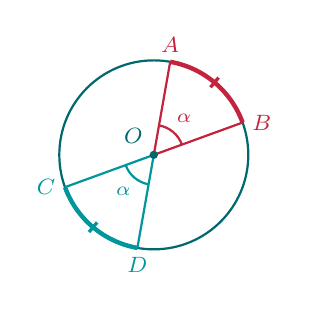
\begin{tikzpicture}[scale=1.0]
      \coordinate (O) at (0,0);
      \draw[thick, color=brandNavy] (O) circle (1.2);
      
      % Sector 1 (AOB)
      \coordinate (A) at (80:1.2);
      \coordinate (B) at (20:1.2);
      \draw[thick, color=brandCrimson] (O) -- (A);
      \draw[thick, color=brandCrimson] (O) -- (B);
      \draw[ultra thick, color=brandCrimson] (20:1.2) arc (20:80:1.2);
      \draw[thick, color=brandCrimson] (20:0.38) arc (20:80:0.38);
      \node[font=\fontsize{7.5}{7.5}\selectfont, color=brandCrimson] at (50:0.6) {$\alpha$};
      \draw[very thick, color=brandCrimson] (50:1.12) -- (50:1.28);
      
      % Sector 2 (COD)
      \coordinate (C) at (200:1.2);
      \coordinate (D) at (260:1.2);
      \draw[thick, color=brandBlue] (O) -- (C);
      \draw[thick, color=brandBlue] (O) -- (D);
      \draw[ultra thick, color=brandBlue] (200:1.2) arc (200:260:1.2);
      \draw[thick, color=brandBlue] (200:0.38) arc (200:260:0.38);
      \node[font=\fontsize{7.5}{7.5}\selectfont, color=brandBlue] at (230:0.6) {$\alpha$};
      \draw[very thick, color=brandBlue] (230:1.12) -- (230:1.28);
      
      % Center and labels
      \fill[brandNavy] (O) circle (1.5pt) node[above left=0.5pt, font=\fontsize{8.5}{8.5}\selectfont] {$O$};
      \node[above, font=\fontsize{8.5}{8.5}\selectfont, color=brandCrimson] at (A) {$A$};
      \node[right, font=\fontsize{8.5}{8.5}\selectfont, color=brandCrimson] at (B) {$B$};
      \node[left, font=\fontsize{8.5}{8.5}\selectfont, color=brandBlue] at (C) {$C$};
      \node[below, font=\fontsize{8.5}{8.5}\selectfont, color=brandBlue] at (D) {$D$};
    \end{tikzpicture}
  \end{minipage}
\end{khboxorange}

\vspace{3pt}
\Needspace*{6.8cm}
\begin{multicols}{2}
  \noindent
  \begin{minipage}{\linewidth}
    \exhead{1} តាមរូបដែលឱ្យខាងក្រោម គេមាន $AB$ ជាអង្កត់ផ្ចិតនៃរង្វង់ផ្ចិត $O$ ហើយធ្នូ $\wideparen{AC} = 30^\circ$ និង $\wideparen{DB} = 80^\circ$ ។\\
    ចូរគណនាតម្លៃនៃ ៖ \quad \khlabel{ក} $\angle COD$ \qquad \khlabel{ខ} $\angle AOD$
    \begin{center}
      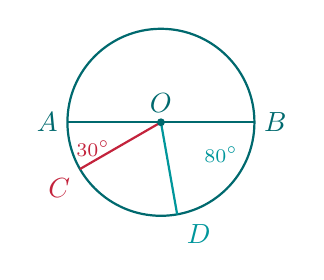
\begin{tikzpicture}[scale=0.95]
        \coordinate (O) at (0,0);
        \draw[thick, color=brandNavy] (O) circle (1.25);
        \coordinate (A) at (-1.25,0);
        \coordinate (B) at (1.25,0);
        \coordinate (C) at ({-1.25*cos(30)},{-1.25*sin(30)});
        \coordinate (D) at ({1.25*cos(80)},{-1.25*sin(80)});
        \draw[thick, color=brandNavy] (A) -- (B);
        \draw[thick, color=brandCrimson] (O) -- (C);
        \draw[thick, color=brandBlue] (O) -- (D);
        \fill[brandNavy] (O) circle (1.5pt) node[above] {$O$};
        \node[left, color=brandNavy] at (A) {$A$};
        \node[right, color=brandNavy] at (B) {$B$};
        \node[below left, color=brandCrimson] at (C) {$C$};
        \node[below right, color=brandBlue] at (D) {$D$};
        \node[below left, font=\fontsize{7.5}{7.5}\selectfont, color=brandCrimson] at (-0.55,-0.12) {$30^\circ$};
        \node[below right, font=\fontsize{7.5}{7.5}\selectfont, color=brandBlue] at (0.45,-0.2) {$80^\circ$};
      \end{tikzpicture}
    \end{center}
  \end{minipage}

  \columnbreak

  \noindent
  \begin{minipage}{\linewidth}
    \exhead{2} តាមរូបដែលឱ្យខាងក្រោម គេមាន $AB$ ជាអង្កត់ផ្ចិតនៃរង្វង់ផ្ចិត $O$ ហើយធ្នូ $\wideparen{AC} = 45^\circ$ និង $\wideparen{DB} = 70^\circ$ ។\\
    ចូរគណនាតម្លៃនៃ ៖ \quad \khlabel{ក} $\angle COD$ \qquad \khlabel{ខ} $\angle AOD$
    \begin{center}
      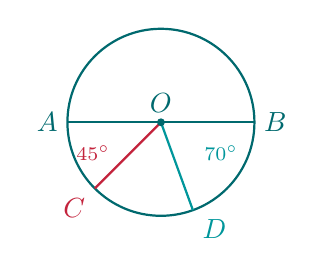
\begin{tikzpicture}[scale=0.95]
        \coordinate (O) at (0,0);
        \draw[thick, color=brandNavy] (O) circle (1.25);
        \coordinate (A) at (-1.25,0);
        \coordinate (B) at (1.25,0);
        \coordinate (C) at ({-1.25*cos(45)},{-1.25*sin(45)});
        \coordinate (D) at ({1.25*cos(70)},{-1.25*sin(70)});
        \draw[thick, color=brandNavy] (A) -- (B);
        \draw[thick, color=brandCrimson] (O) -- (C);
        \draw[thick, color=brandBlue] (O) -- (D);
        \fill[brandNavy] (O) circle (1.5pt) node[above] {$O$};
        \node[left, color=brandNavy] at (A) {$A$};
        \node[right, color=brandNavy] at (B) {$B$};
        \node[below left, color=brandCrimson] at (C) {$C$};
        \node[below right, color=brandBlue] at (D) {$D$};
        \node[below left, font=\fontsize{7.5}{7.5}\selectfont, color=brandCrimson] at (-0.55,-0.18) {$45^\circ$};
        \node[below right, font=\fontsize{7.5}{7.5}\selectfont, color=brandBlue] at (0.45,-0.18) {$70^\circ$};
      \end{tikzpicture}
    \end{center}
  \end{minipage}
\end{multicols}

\vspace{1pt}
\Needspace*{6.8cm}
\begin{multicols}{2}
  \noindent
  \begin{minipage}{\linewidth}
    \exhead{3} នៅក្នុងរង្វង់ផ្ចិត $O$ គេឱ្យអង្កត់ផ្ចិត $AD$ ហើយ $C$ ជាចំណុចមួយនៃធ្នូ $\wideparen{BD}$ ដែលធ្នូ $\wideparen{AB} = 40^\circ$ និងធ្នូ $\wideparen{CD} = 60^\circ$ ។\\
    ចូរគណនារង្វាស់នៃ $\angle AOC$ ៖
    \begin{center}
      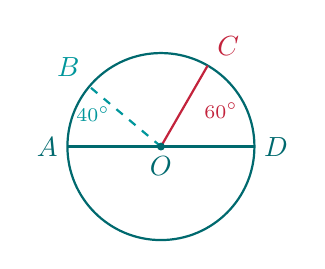
\begin{tikzpicture}[scale=0.95]
        \coordinate (O) at (0,0);
        \draw[thick, color=brandNavy] (O) circle (1.25);
        \coordinate (A) at (-1.25,0);
        \coordinate (D) at (1.25,0);
        \coordinate (B) at ({-1.25*cos(40)},{1.25*sin(40)});
        \coordinate (C) at ({1.25*cos(60)},{1.25*sin(60)});
        \draw[thick, color=brandNavy] (A) -- (D);
        \draw[thick, dashed, color=brandTeal] (O) -- (B);
        \draw[thick, color=brandCrimson] (O) -- (C);
        \fill[brandNavy] (O) circle (1.5pt) node[below] {$O$};
        \node[left, color=brandNavy] at (A) {$A$};
        \node[right, color=brandNavy] at (D) {$D$};
        \node[above left, color=brandTeal] at (B) {$B$};
        \node[above right, color=brandCrimson] at (C) {$C$};
        \node[above left, font=\fontsize{7.5}{7.5}\selectfont, color=brandTeal] at (-0.55,0.2) {$40^\circ$};
        \node[above right, font=\fontsize{7.5}{7.5}\selectfont, color=brandCrimson] at (0.45,0.25) {$60^\circ$};
      \end{tikzpicture}
    \end{center}
  \end{minipage}

  \columnbreak

  \noindent
  \begin{minipage}{\linewidth}
    \exhead{4} គេឱ្យរង្វង់ផ្ចិត $O$ និង $B$ ជាចំណុចកណ្ដាលនៃធ្នូ $\wideparen{AC}$ ដែលមានរង្វាស់ធ្នូ $\wideparen{AC} = 100^\circ$ ។\\
    \khlabel{ក} ចូរបង្ហាញថា $\angle AOB = \angle COB$ ។\\
    \khlabel{ខ} គណនារង្វាស់នៃមុំ $\angle AOB$ និង $\angle COB$ ។
    \begin{center}
      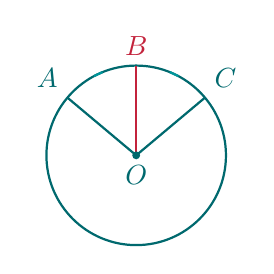
\begin{tikzpicture}[scale=0.95]
        \coordinate (O) at (0,0);
        \draw[thick, color=brandNavy] (O) circle (1.2);
        \coordinate (A) at (140:1.2);
        \coordinate (B) at (90:1.2);
        \coordinate (C) at (40:1.2);
        \draw[thick, color=brandNavy] (O) -- (A);
        \draw[thick, color=brandCrimson] (O) -- (B);
        \draw[thick, color=brandNavy] (O) -- (C);
        \fill[brandNavy] (O) circle (1.5pt) node[below] {$O$};
        \node[above left, color=brandNavy] at (A) {$A$};
        \node[above, color=brandCrimson] at (B) {$B$};
        \node[above right, color=brandNavy] at (C) {$C$};
        \draw[color=brandTeal, thick] (112:1.2) -- (118:1.2);
        \draw[color=brandTeal, thick] (62:1.2) -- (68:1.2);
      \end{tikzpicture}
    \end{center}
  \end{minipage}
\end{multicols}

% =========================================================================
% SECTION 2: មុំចារឹកក្នុងរង្វង់
% =========================================================================
\vspace{6pt}
\khsection{២}{មុំចារឹកក្នុងរង្វង់}

\khsubsection{២.១}{និយមន័យ}

\begin{khboxorange}
  \begin{minipage}[c]{0.70\textwidth}
    \textbf{មុំចារឹកក្នុងរង្វង់ជាមុំដែលមានកំពូលស្ថិតនៅលើរង្វង់ ហើយជ្រុងទាំងពីរកាត់រង្វង់ជាអង្កត់ធ្នូ ៖}
    \begin{itemize}[leftmargin=12pt, itemsep=1pt, topsep=1pt, parsep=0pt]
      \item[\color{brandCrimson}\ding{228}] កំពូល $A$ ស្ថិតនៅលើរង្វង់ផ្ចិត $O$
      \item[\color{brandNavy}\ding{228}] ជ្រុង $AB$ និង $AC$ ជាអង្កត់ធ្នូនៃរង្វង់
      \item[\color{brandTeal}\ding{228}] $\angle BAC$ ជា\textbf{មុំចារឹកក្នុងរង្វង់} ស្ទាក់ធ្នូ $\wideparen{BC}$
    \end{itemize}
  \end{minipage}\hfill
  \begin{minipage}[c]{0.28\textwidth}
    \centering
    \begin{tikzpicture}[scale=0.88]
      \coordinate (O) at (0,0);
      \draw[thick, color=brandNavy] (O) circle (1.1);
      \coordinate (A) at (90:1.1);
      \coordinate (B) at (215:1.1);
      \coordinate (C) at (-35:1.1);
      \draw[thick, color=brandCrimson] (B) -- (A) -- (C);
      \draw[ultra thick, color=brandTeal] (-35:1.1) arc (-35:-145:1.1);
      \fill[brandNavy] (O) circle (1.5pt) node[below=1pt, font=\fontsize{8}{8}\selectfont] {$O$};
      \node[above=1pt, font=\fontsize{8.5}{8.5}\selectfont, color=brandCrimson] at (A) {$A$};
      \node[below left=1pt, font=\fontsize{8.5}{8.5}\selectfont, color=brandNavy] at (B) {$B$};
      \node[below right=1pt, font=\fontsize{8.5}{8.5}\selectfont, color=brandNavy] at (C) {$C$};
      \draw[thick, color=brandCrimson] ([shift=(-125:0.28)]A) arc (-125:-55:0.28);
      \node[below=1pt, font=\fontsize{7.5}{7.5}\selectfont, color=brandTeal] at (0,-1.15) {ធ្នូស្ទាក់ $\wideparen{BC}$};
    \end{tikzpicture}
  \end{minipage}
\end{khboxorange}

\vspace{2pt}
\begin{khcard}
  \exhead{5} តើមុំខាងក្រោមនេះជាមុំចារឹកក្នុងរង្វង់ឬទេ? ព្រោះអ្វី?
  \par\vspace{2pt}
  \centerline{\begin{tikzpicture}[scale=0.80]
      % Figure 1
      \begin{scope}[xshift=0cm]
        \coordinate (O1) at (0,0);
        \draw[thick, color=brandNavy] (O1) circle (1.0);
        \coordinate (A1) at (30:1.0);
        \coordinate (X1) at (150:1.0);
        \coordinate (Y1) at (230:1.0);
        \draw[thick, color=brandCrimson] (X1) -- (A1) -- (Y1);
        \fill[brandNavy] (O1) circle (1.5pt) node[below left] {$O$};
        \node[above right, color=brandCrimson] at (A1) {$A$};
        \node[above left] at (X1) {$x$};
        \node[below left] at (Y1) {$y$};
        \node[below] at (0,-1.2) {\khlabel{ក}};
      \end{scope}

      % Figure 2
      \begin{scope}[xshift=5.8cm]
        \coordinate (O2) at (0,0);
        \draw[thick, color=brandNavy] (O2) circle (1.0);
        \coordinate (A2) at (90:1.0);
        \coordinate (X2) at (210:1.0);
        \coordinate (Y2) at (330:1.0);
        \draw[thick, color=brandCrimson] (X2) -- (A2) -- (Y2);
        \fill[brandNavy] (O2) circle (1.5pt) node[below] {$O$};
        \node[above, color=brandCrimson] at (A2) {$A$};
        \node[below left] at (X2) {$x$};
        \node[below right] at (Y2) {$y$};
        \node[below] at (0,-1.2) {\khlabel{ខ}};
      \end{scope}

      % Figure 3
      \begin{scope}[xshift=11.6cm]
        \coordinate (O3) at (0,0);
        \draw[thick, color=brandNavy] (O3) circle (1.0);
        \coordinate (A3) at (90:1.0);
        \coordinate (X3) at (270:1.0);
        \coordinate (Y3) at (1.7,0.65);
        \draw[thick, color=brandCrimson] (X3) -- (A3) -- (Y3);
        \fill[brandNavy] (O3) circle (1.5pt) node[left] {$O$};
        \node[above, color=brandCrimson] at (A3) {$A$};
        \node[left=1pt] at (X3) {$x$};
        \node[right] at (Y3) {$y$};
        \node[below] at (0,-1.2) {\khlabel{គ}};
      \end{scope}
    \end{tikzpicture}}
  \vspace{1pt}
\end{khcard}

\vspace{2pt}
\Needspace*{4.2cm}
\begin{multicols}{2}
  \noindent
  \begin{minipage}{\linewidth}
    \exhead{6} តាមរូបខាងស្ដាំនេះ គេមានរង្វង់ផ្ចិតមួយ និងអង្កត់ធ្នូនានាគូសចេញពី $P$ ។\\
    តើក្នុងរូបនេះមានមុំចារឹកក្នុងរង្វង់ចំនួនប៉ុន្មាន? ចូរបញ្ជាក់ឈ្មោះមុំនីមួយៗ ។
    \par\vspace{2pt}
    \centerline{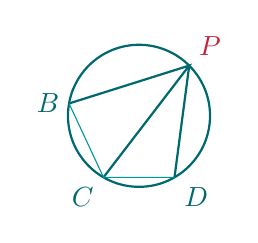
\begin{tikzpicture}[scale=0.82]
        \draw[thick, color=brandNavy] (0,0) circle (1.1);
        \coordinate (P) at (45:1.1);
        \coordinate (B) at (170:1.1);
        \coordinate (C) at (240:1.1);
        \coordinate (D) at (300:1.1);
        \draw[thick, color=brandNavy] (B) -- (P) -- (C);
        \draw[thick, color=brandNavy] (P) -- (D);
        \draw[color=brandTeal] (B) -- (C) -- (D);
        \node[above right, color=brandCrimson] at (P) {$P$};
        \node[left, color=brandNavy] at (B) {$B$};
        \node[below left, color=brandNavy] at (C) {$C$};
        \node[below right, color=brandNavy] at (D) {$D$};
      \end{tikzpicture}}
  \end{minipage}

  \columnbreak

  \noindent
  \begin{minipage}{\linewidth}
    \exhead{7} តាមរូបខាងស្ដាំនេះ គេមានត្រីកោណ $ABC$ ចារឹកក្នុងរង្វង់ និងអង្កត់ធ្នូ $AD$ គូសបន្ថែម ។\\
    ចូរកំណត់ឈ្មោះមុំចារឹកទាំងអស់ដែលមានកំពូលត្រង់ $A$ និងបញ្ជាក់ធ្នូស្ទាក់នៃមុំនីមួយៗ ។
    \par\vspace{2pt}
    \centerline{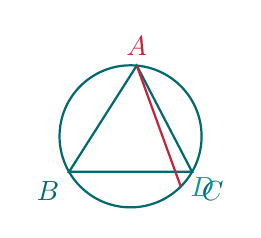
\begin{tikzpicture}[scale=0.82]
        \draw[thick, color=brandNavy] (0,0) circle (1.1);
        \coordinate (A) at (85:1.1);
        \coordinate (B) at (210:1.1);
        \coordinate (C) at (330:1.1);
        \coordinate (D) at (-45:1.1);
        \draw[thick, color=brandNavy] (A) -- (B) -- (C) -- cycle;
        \draw[thick, color=brandCrimson] (A) -- (D);
        \node[above, color=brandCrimson] at (A) {$A$};
        \node[below left, color=brandNavy] at (B) {$B$};
        \node[below right, color=brandNavy] at (C) {$C$};
        \node[right, color=brandTeal] at (D) {$D$};
      \end{tikzpicture}}
  \end{minipage}
\end{multicols}

% =========================================================================
% SECTION 2.2: មុំចារឹកក្នុងរង្វង់ និងធ្នូ
% =========================================================================
\vspace{3pt}
\khsubsection{២.២}{មុំចារឹកក្នុងរង្វង់ និងធ្នូ}

\begin{khboxorange}
  \begin{minipage}[c]{0.70\textwidth}
    \raggedright
    \textbf{គ្រប់មុំចារឹកក្នុងរង្វង់មានរង្វាស់ស្មើនឹងកន្លះរង្វាស់ធ្នូដែលស្ទាក់មុំនោះ ៖}
    \begin{itemize}[leftmargin=12pt, itemsep=1pt, topsep=1pt, parsep=0pt]
      \item[\color{brandCrimson}\ding{228}] រង្វាស់មុំចារឹកស្មើពាក់កណ្ដាលរង្វាស់ធ្នូស្ទាក់
      \item[\color{brandBlue}\ding{228}] រង្វាស់មុំចារឹកស្មើពាក់កណ្ដាលមុំផ្ចិតស្ទាក់ធ្នូរួម
    \end{itemize}
    \vspace{2pt}
    \centerline{\koreahl{$\angle ABC = \frac{1}{2}\wideparen{AC} = \frac{1}{2}\angle AOC$}}
  \end{minipage}\hfill
  \begin{minipage}[c]{0.28\textwidth}
    \centering
    \begin{tikzpicture}[scale=0.80]
      \coordinate (O) at (0,0);
      \draw[thick, color=brandNavy] (O) circle (1.0);
      \coordinate (B) at (105:1.0);
      \coordinate (A) at (215:1.0);
      \coordinate (C) at (-25:1.0);
      \draw[thick, color=brandCrimson] (A) -- (B) -- (C);
      \draw[thick, color=brandBlue] (A) -- (O) -- (C);
      \draw[ultra thick, color=brandTeal] (-25:1.0) arc (-25:-145:1.0);
      \fill[brandNavy] (O) circle (1.5pt) node[above=2pt, font=\fontsize{7.5}{7.5}\selectfont] {$O$};
      \node[above, font=\fontsize{8}{8}\selectfont, color=brandCrimson] at (B) {$B$};
      \node[left, font=\fontsize{8}{8}\selectfont, color=brandNavy] at (A) {$A$};
      \node[right, font=\fontsize{8}{8}\selectfont, color=brandNavy] at (C) {$C$};
      \draw[thick, color=brandCrimson] ([shift=(244:0.32)]B) arc (244:294:0.32);
      \draw[thick, color=brandBlue] ([shift=(215:0.28)]O) arc (215:335:0.28);
      \node[font=\fontsize{7}{7}\selectfont, color=brandCrimson] at ($(B)+(-65:0.42)$) {$\alpha$};
      \node[font=\fontsize{7}{7}\selectfont, color=brandBlue] at ($(O)+(-85:0.38)$) {$2\alpha$};
      \node[below=1pt, font=\fontsize{7}{7}\selectfont, color=brandTeal] at (0,-1.02) {ធ្នូ $\wideparen{AC}$};
    \end{tikzpicture}
  \end{minipage}
\end{khboxorange}

\vspace{2pt}
\Needspace*{4.2cm}
\begin{multicols}{2}
  \noindent
  \begin{minipage}{\linewidth}
    \exhead{8} គេឱ្យ $\angle ABC$ ជាមុំចារឹកក្នុងរង្វង់ផ្ចិត $O$ ដែលមាន $BC$ ជាអង្កត់ផ្ចិត (ដូចរូប) ។\\
    ចូរបង្ហាញថា ៖ \quad $\angle ABC = \frac{1}{2}\wideparen{AC}$
    \par\vspace{2pt}
    \centerline{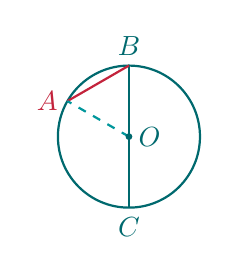
\begin{tikzpicture}[scale=0.82]
        \coordinate (O) at (0,0);
        \draw[thick, color=brandNavy] (O) circle (1.1);
        \coordinate (B) at (90:1.1);
        \coordinate (C) at (-90:1.1);
        \coordinate (A) at (150:1.1);
        \draw[thick, color=brandNavy] (B) -- (C);
        \draw[thick, color=brandCrimson] (B) -- (A);
        \draw[thick, dashed, color=brandTeal] (O) -- (A);
        \fill[brandNavy] (O) circle (1.5pt) node[right] {$O$};
        \node[above, color=brandNavy] at (B) {$B$};
        \node[below, color=brandNavy] at (C) {$C$};
        \node[left, color=brandCrimson] at (A) {$A$};
      \end{tikzpicture}}
  \end{minipage}

  \columnbreak

  \noindent
  \begin{minipage}{\linewidth}
    \exhead{9} តាមរូបខាងស្ដាំ គេមានត្រីកោណ $ABC$ ចារឹកក្នុងរង្វង់ ដោយស្គាល់ $\angle A = 40^\circ$, $\angle B = 60^\circ$ និង $\angle C = 80^\circ$ ។\\
    ចូរគណនារង្វាស់ធ្នូ $\wideparen{BC}$, $\wideparen{AC}$, និង $\wideparen{AB}$ ៖
    \par\vspace{2pt}
    \centerline{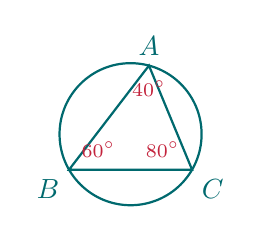
\begin{tikzpicture}[scale=0.82]
        \coordinate (O) at (0,0);
        \draw[thick, color=brandNavy] (O) circle (1.1);
        \coordinate (A) at (75:1.1);
        \coordinate (B) at (210:1.1);
        \coordinate (C) at (330:1.1);
        \draw[thick, color=brandNavy] (A) -- (B) -- (C) -- cycle;
        \node[above, color=brandNavy] at (A) {$A$};
        \node[below left, color=brandNavy] at (B) {$B$};
        \node[below right, color=brandNavy] at (C) {$C$};
        \node[below=2pt, font=\fontsize{7.5}{7.5}\selectfont, color=brandCrimson] at (A) {$40^\circ$};
        \node[above right=1pt, font=\fontsize{7.5}{7.5}\selectfont, color=brandCrimson] at (B) {$60^\circ$};
        \node[above left=1pt, font=\fontsize{7.5}{7.5}\selectfont, color=brandCrimson] at (C) {$80^\circ$};
      \end{tikzpicture}}
  \end{minipage}
\end{multicols}

\vspace{1pt}
\Needspace*{4.2cm}
\begin{multicols}{2}
  \noindent
  \begin{minipage}{\linewidth}
    \exhead{10} តាមរូបខាងស្ដាំ គេមានត្រីកោណ $ABC$ ចារឹកក្នុងរង្វង់ ដោយស្គាល់ $\angle A = 50^\circ$, $\angle B = 70^\circ$ និង $\angle C = 60^\circ$ ។\\
    ចូរគណនារង្វាស់ធ្នូ $\wideparen{BC}$, $\wideparen{AC}$, និង $\wideparen{AB}$ ៖
    \par\vspace{2pt}
    \centerline{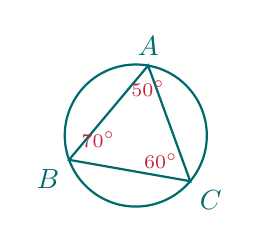
\begin{tikzpicture}[scale=0.82]
        \coordinate (O) at (0,0);
        \draw[thick, color=brandNavy] (O) circle (1.1);
        \coordinate (A) at (80:1.1);
        \coordinate (B) at (200:1.1);
        \coordinate (C) at (320:1.1);
        \draw[thick, color=brandNavy] (A) -- (B) -- (C) -- cycle;
        \node[above, color=brandNavy] at (A) {$A$};
        \node[below left, color=brandNavy] at (B) {$B$};
        \node[below right, color=brandNavy] at (C) {$C$};
        \node[below=2pt, font=\fontsize{7.5}{7.5}\selectfont, color=brandCrimson] at (A) {$50^\circ$};
        \node[above right=1pt, font=\fontsize{7.5}{7.5}\selectfont, color=brandCrimson] at (B) {$70^\circ$};
        \node[above left=1pt, font=\fontsize{7.5}{7.5}\selectfont, color=brandCrimson] at (C) {$60^\circ$};
      \end{tikzpicture}}
  \end{minipage}

  \columnbreak

  \noindent
  \begin{minipage}{\linewidth}
    \exhead{11} ត្រីកោណ $MNP$ ជាត្រីកោណចារឹកក្នុងរង្វង់ផ្ចិត $O$ ដែលមានរង្វាស់ធ្នូ $\wideparen{MN} = 100^\circ$ និង $\wideparen{NP} = 140^\circ$ ។\\
    ចូរគណនារង្វាស់មុំនីមួយៗនៃត្រីកោណ $MNP$ នេះ ៖
    \par\vspace{2pt}
    \centerline{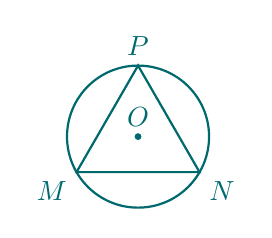
\begin{tikzpicture}[scale=0.82]
        \coordinate (O) at (0,0);
        \draw[thick, color=brandNavy] (O) circle (1.1);
        \coordinate (P) at (90:1.1);
        \coordinate (M) at (210:1.1);
        \coordinate (N) at (330:1.1);
        \draw[thick, color=brandNavy] (M) -- (N) -- (P) -- cycle;
        \fill[brandNavy] (O) circle (1.5pt) node[above] {$O$};
        \node[above, color=brandNavy] at (P) {$P$};
        \node[below left, color=brandNavy] at (M) {$M$};
        \node[below right, color=brandNavy] at (N) {$N$};
      \end{tikzpicture}}
  \end{minipage}
\end{multicols}

\vspace{1pt}
\Needspace*{4.2cm}
\begin{multicols}{2}
  \noindent
  \begin{minipage}{\linewidth}
    \exhead{12} ត្រីកោណ $MNP$ ជាត្រីកោណចារឹកក្នុងរង្វង់ផ្ចិត $O$ ដែលមានរង្វាស់ធ្នូ $\wideparen{MN} = 110^\circ$ និង $\wideparen{NP} = 130^\circ$ ។\\
    ចូរគណនារង្វាស់មុំនីមួយៗនៃត្រីកោណ $MNP$ នេះ ៖
    \par\vspace{1pt}
    \centerline{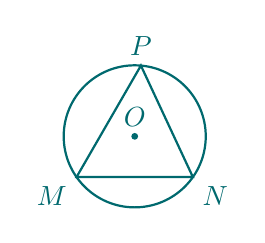
\begin{tikzpicture}[scale=0.82]
        \coordinate (O) at (0,0);
        \draw[thick, color=brandNavy] (O) circle (1.1);
        \coordinate (P) at (85:1.1);
        \coordinate (M) at (215:1.1);
        \coordinate (N) at (325:1.1);
        \draw[thick, color=brandNavy] (M) -- (N) -- (P) -- cycle;
        \fill[brandNavy] (O) circle (1.5pt) node[above] {$O$};
        \node[above, color=brandNavy] at (P) {$P$};
        \node[below left, color=brandNavy] at (M) {$M$};
        \node[below right, color=brandNavy] at (N) {$N$};
      \end{tikzpicture}}
  \end{minipage}

  \columnbreak

  \noindent
  \begin{minipage}{\linewidth}
    \exhead{13} គេមាន $\angle ABC$ ចារឹកក្នុងរង្វង់ផ្ចិត $O$ ដែល\\
    $O$ ស្ថិតនៅក្រៅ $\angle ABC$ ។ ដោយប្រើលក្ខណៈនៃ\\
    លំហាត់ទី ៨ ចូរបង្ហាញថា ៖{\koreahl{$\angle ABC = \frac{1}{2}\wideparen{AC}$}}
    \par
    \centerline{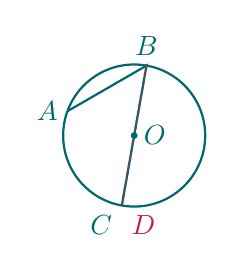
\begin{tikzpicture}[scale=0.82]
        \coordinate (O) at (0,0);
        \draw[thick, color=brandNavy] (O) circle (1.1);
        \coordinate (B) at (80:1.1);
        \coordinate (A) at (160:1.1);
        \coordinate (C) at (260:1.1);
        \coordinate (D) at (-100:1.1);
        \draw[thick, color=brandNavy] (A) -- (B) -- (C);
        \draw[thick, dotted, color=brandCrimson] (B) -- (D);
        \fill[brandNavy] (O) circle (1.5pt) node[right] {$O$};
        \node[above, color=brandNavy] at (B) {$B$};
        \node[left, color=brandNavy] at (A) {$A$};
        \node[below left, color=brandNavy] at (C) {$C$};
        \node[below right, color=brandCrimson] at (D) {$D$};
      \end{tikzpicture}}
  \end{minipage}
\end{multicols}

% =========================================================================
% SECTION 2.3: មុំចារឹកក្នុងរង្វង់ស្ទាក់ធ្នូតែមួយ
% =========================================================================
\vspace{-0.5cm}
\khsubsection{២.៣}{មុំចារឹកក្នុងរង្វង់ស្ទាក់ធ្នូតែមួយ}
\begin{khboxorange}
  \begin{minipage}[c]{0.70\textwidth}
    \raggedright
    \begin{itemize}[leftmargin=12pt, itemsep=1pt, topsep=1pt, parsep=0pt]
      \item[\color{brandNavy}\ding{228}] \textbf{គ្រប់មុំចារឹកក្នុងរង្វង់មានរង្វាស់ស្មើនឹងកន្លះរង្វាស់ធ្នូដែលស្ទាក់មុំនោះ ។}
      \item[\color{brandCrimson}\ding{228}] \textbf{គ្រប់មុំចារឹកក្នុងរង្វង់ដែលស្ទាក់ធ្នូតែមួយមានរង្វាស់ស្មើគ្នា ៖ {\koreahl{$\angle ACB = \angle ADB = \frac{1}{2}\wideparen{AB}$}}}
    \end{itemize}
  
  \end{minipage}\hfill
  \begin{minipage}[c]{0.28\textwidth}
    \centering
    \begin{tikzpicture}[scale=0.80]
      \coordinate (O) at (0,0);
      \draw[thick, color=brandNavy] (O) circle (1.0);
      \coordinate (A) at (215:1.0);
      \coordinate (B) at (-35:1.0);
      \coordinate (C) at (130:1.0);
      \coordinate (D) at (50:1.0);
      \draw[thick, color=brandCrimson] (A) -- (C) -- (B);
      \draw[thick, color=brandBlue] (A) -- (D) -- (B);
      \draw[ultra thick, color=brandTeal] (-35:1.0) arc (-35:-145:1.0);
      \fill[brandNavy] (O) circle (1.5pt) node[below=1pt, font=\fontsize{7.5}{7.5}\selectfont] {$O$};
      \node[left, font=\fontsize{8}{8}\selectfont, color=brandNavy] at (A) {$A$};
      \node[right, font=\fontsize{8}{8}\selectfont, color=brandNavy] at (B) {$B$};
      \node[above left, font=\fontsize{8}{8}\selectfont, color=brandCrimson] at (C) {$C$};
      \node[above right, font=\fontsize{8}{8}\selectfont, color=brandBlue] at (D) {$D$};
      \draw[thick, color=brandCrimson] ([shift=(244:0.32)]C) arc (244:296:0.32);
      \draw[thick, color=brandBlue] ([shift=(236:0.32)]D) arc (236:284:0.32);
      \node[font=\fontsize{7}{7}\selectfont, color=brandCrimson] at ($(C)+(-70:0.42)$) {$\alpha$};
      \node[font=\fontsize{7}{7}\selectfont, color=brandBlue] at ($(D)+(-110:0.42)$) {$\alpha$};
      \node[below=1pt, font=\fontsize{7}{7}\selectfont, color=brandTeal] at (0,-1.02) {ធ្នូ $\wideparen{AB}$};
    \end{tikzpicture}
  \end{minipage}
\end{khboxorange}


\Needspace*{4.0cm}
\begin{multicols}{2}
  \noindent
  \begin{minipage}{\linewidth}
    \exhead{14} តាមរូបខាងស្ដាំនេះ ចូររករង្វាស់មុំ $a$ និង $b$ ៖
    \par\vspace{1pt}
    \centerline{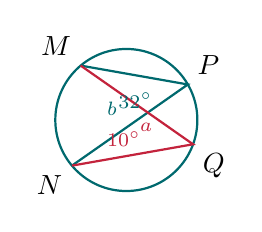
\begin{tikzpicture}[scale=0.82]
        \coordinate (O) at (0,0);
        \draw[thick, color=brandNavy] (O) circle (1.1);
        \coordinate (M) at (130:1.1);
        \coordinate (N) at (220:1.1);
        \coordinate (P) at (30:1.1);
        \coordinate (Q) at (-20:1.1);
        \draw[thick, color=brandNavy] (M) -- (P) -- (N);
        \draw[thick, color=brandCrimson] (M) -- (Q) -- (N);
        \node[above left] at (M) {$M$};
        \node[below left] at (N) {$N$};
        \node[above right] at (P) {$P$};
        \node[below right] at (Q) {$Q$};
        \node[left, font=\fontsize{7.5}{7.5}\selectfont, color=brandNavy] at (0.55,0.3) {$32^\circ$};
        \node[left, font=\fontsize{7.5}{7.5}\selectfont, color=brandCrimson] at (0.55,-0.12) {$a$};
        \node[right, font=\fontsize{7.5}{7.5}\selectfont, color=brandNavy] at (-0.45,0.18) {$b$};
        \node[right, font=\fontsize{7.5}{7.5}\selectfont, color=brandCrimson] at (-0.45,-0.3) {$10^\circ$};
      \end{tikzpicture}}
  \end{minipage}

  \columnbreak

  \noindent
  \begin{minipage}{\linewidth}
    \exhead{15} តាមរូបខាងស្ដាំនេះ ចូររករង្វាស់មុំ $a$ និង $b$ ៖
    \par\vspace{1pt}
    \centerline{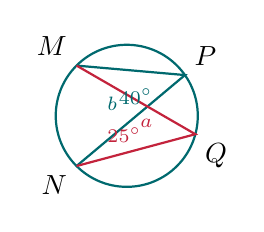
\begin{tikzpicture}[scale=0.82]
        \coordinate (O) at (0,0);
        \draw[thick, color=brandNavy] (O) circle (1.1);
        \coordinate (M) at (135:1.1);
        \coordinate (N) at (225:1.1);
        \coordinate (P) at (35:1.1);
        \coordinate (Q) at (-15:1.1);
        \draw[thick, color=brandNavy] (M) -- (P) -- (N);
        \draw[thick, color=brandCrimson] (M) -- (Q) -- (N);
        \node[above left] at (M) {$M$};
        \node[below left] at (N) {$N$};
        \node[above right] at (P) {$P$};
        \node[below right] at (Q) {$Q$};
        \node[left, font=\fontsize{7.5}{7.5}\selectfont, color=brandNavy] at (0.55,0.3) {$40^\circ$};
        \node[left, font=\fontsize{7.5}{7.5}\selectfont, color=brandCrimson] at (0.55,-0.12) {$a$};
        \node[right, font=\fontsize{7.5}{7.5}\selectfont, color=brandNavy] at (-0.45,0.18) {$b$};
        \node[right, font=\fontsize{7.5}{7.5}\selectfont, color=brandCrimson] at (-0.45,-0.3) {$25^\circ$};
      \end{tikzpicture}}
  \end{minipage}
\end{multicols}


%\Needspace*{4.0cm}
\begin{multicols}{2}
  \noindent
  \begin{minipage}{\linewidth}
    \exhead{16} គេឱ្យអង្កត់ធ្នូ $BD = DC$, $\angle ABD = 42^\circ$ និង $\angle DBC = 65^\circ$ (ដូចរូប) ។ ចូរគណនា ៖\\
    \khlabel{ក} $\angle BDC$ \qquad \khlabel{ខ} $\angle BAC$ \\
    \khlabel{គ} $\angle DAB$ \qquad \khlabel{ឃ} $\angle DEC$
    \par\vspace{1pt}
    \centerline{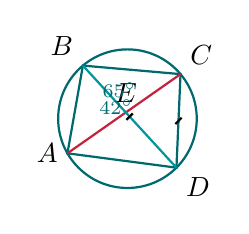
\begin{tikzpicture}[scale=0.80]
        \coordinate (O) at (0,0);
        \draw[thick, color=brandNavy] (O) circle (1.1);
        \coordinate (A) at (210:1.1);
        \coordinate (B) at (130:1.1);
        \coordinate (C) at (40:1.1);
        \coordinate (D) at (-45:1.1);
        \draw[thick, color=brandNavy] (A) -- (B) -- (C) -- (D) -- cycle;
        \draw[thick, color=brandCrimson] (A) -- (C);
        \draw[thick, color=brandTeal] (B) -- (D);
        \coordinate (E) at (intersection of A--C and B--D);
        \node[left] at (A) {$A$};
        \node[above left] at (B) {$B$};
        \node[above right] at (C) {$C$};
        \node[below right] at (D) {$D$};
        \node[above] at (E) {$E$};
        \node[right, font=\fontsize{7}{7}\selectfont, color=brandNavy] at (-0.55,0.45) {$65^\circ$};
        \node[right, font=\fontsize{7}{7}\selectfont, color=brandNavy] at (-0.6,0.18) {$42^\circ$};
        \draw[thick] ($(B)!0.5!(D)$) ++(-0.05,-0.05) -- ++(0.1,0.1);
        \draw[thick] ($(C)!0.5!(D)$) ++(-0.05,-0.05) -- ++(0.1,0.1);
      \end{tikzpicture}}
  \end{minipage}

  \columnbreak

  \noindent
  \begin{minipage}{\linewidth}
    \exhead{17} ក្នុងរូបខាងស្ដាំនេះ អង្កត់ធ្នូ $AC$ ប្រសព្វនឹង $BD$ ត្រង់ $I$ ។ គេឱ្យ $\angle ACB = 34^\circ$ និង $\angle CAD = 45^\circ$ ។\\
    ចូរគណនារង្វាស់មុំ $\angle AIB$ ៖
    \par\vspace{1pt}
    \centerline{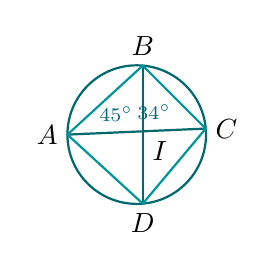
\begin{tikzpicture}[scale=0.80]
        \coordinate (O) at (0,0);
        \draw[thick, color=brandNavy] (O) circle (1.1);
        \coordinate (A) at (180:1.1);
        \coordinate (B) at (85:1.1);
        \coordinate (C) at (5:1.1);
        \coordinate (D) at (-85:1.1);
        \draw[thick, color=brandNavy] (A) -- (C);
        \draw[thick, color=brandNavy] (B) -- (D);
        \draw[thick, color=brandTeal] (A) -- (B) -- (C) -- (D) -- cycle;
        \coordinate (I) at (intersection of A--C and B--D);
        \node[left] at (A) {$A$};
        \node[above] at (B) {$B$};
        \node[right] at (C) {$C$};
        \node[below] at (D) {$D$};
        \node[below right] at (I) {$I$};
        \node[above right, font=\fontsize{7}{7}\selectfont, color=brandNavy] at (-0.75,0.05) {$45^\circ$};
        \node[above left, font=\fontsize{7}{7}\selectfont, color=brandNavy] at (0.7,0.08) {$34^\circ$};
      \end{tikzpicture}}
  \end{minipage}
\end{multicols}

\begin{multicols}{2}
  \noindent
  \begin{minipage}{\linewidth}
    \exhead{18} ក្នុងរូបខាងស្ដាំនេះ អង្កត់ធ្នូ $AC$ ប្រសព្វនឹង $BD$ ត្រង់ $I$ ។ គេឱ្យ $\angle ACB = 30^\circ$ និង $\angle CAD = 50^\circ$ ។\\
    ចូរគណនារង្វាស់មុំ $\angle AIB$ ៖
    \par\vspace{1pt}
    \centerline{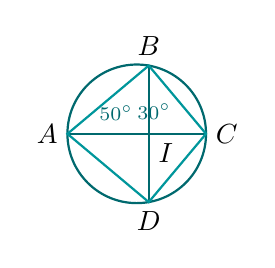
\begin{tikzpicture}[scale=0.80]
        \coordinate (O) at (0,0);
        \draw[thick, color=brandNavy] (O) circle (1.1);
        \coordinate (A) at (180:1.1);
        \coordinate (B) at (80:1.1);
        \coordinate (C) at (0:1.1);
        \coordinate (D) at (-80:1.1);
        \draw[thick, color=brandNavy] (A) -- (C);
        \draw[thick, color=brandNavy] (B) -- (D);
        \draw[thick, color=brandTeal] (A) -- (B) -- (C) -- (D) -- cycle;
        \coordinate (I) at (intersection of A--C and B--D);
        \node[left] at (A) {$A$};
        \node[above] at (B) {$B$};
        \node[right] at (C) {$C$};
        \node[below] at (D) {$D$};
        \node[below right] at (I) {$I$};
        \node[above right, font=\fontsize{7}{7}\selectfont, color=brandNavy] at (-0.75,0.05) {$50^\circ$};
        \node[above left, font=\fontsize{7}{7}\selectfont, color=brandNavy] at (0.7,0.08) {$30^\circ$};
      \end{tikzpicture}}
  \end{minipage}

  \columnbreak

  \noindent
  \begin{minipage}{\linewidth}
    \exhead{19} តាមរូបខាងស្ដាំនេះ គេឱ្យ $\angle BAC = 45^\circ$ និង $\angle BEC = 130^\circ$ ។\\
    ចូររករង្វាស់មុំ $\angle ACD$, $\angle BAE$, និង $\angle BDC$ ៖
    \par\vspace{1pt}
    \centerline{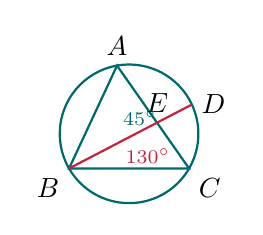
\begin{tikzpicture}[scale=0.80]
        \coordinate (O) at (0,0);
        \draw[thick, color=brandNavy] (O) circle (1.1);
        \coordinate (A) at (100:1.1);
        \coordinate (B) at (210:1.1);
        \coordinate (C) at (-30:1.1);
        \coordinate (D) at (25:1.1);
        \draw[thick, color=brandNavy] (A) -- (B) -- (C) -- cycle;
        \draw[thick, color=brandCrimson] (B) -- (D);
        \coordinate (E) at (intersection of A--C and B--D);
        \node[above] at (A) {$A$};
        \node[below left] at (B) {$B$};
        \node[below right] at (C) {$C$};
        \node[right] at (D) {$D$};
        \node[above] at (E) {$E$};
        \node[right, font=\fontsize{7}{7}\selectfont, color=brandNavy] at (-0.25,0.25) {$45^\circ$};
        \node[below, font=\fontsize{7}{7}\selectfont, color=brandCrimson] at (0.3,-0.08) {$130^\circ$};
      \end{tikzpicture}}
  \end{minipage}
\end{multicols}

\begin{khcard}
  \begin{minipage}[c]{0.72\textwidth}
    \exhead{20} ក្នុងរង្វង់ផ្ចិត $O$ គេឱ្យអង្កត់ធ្នូ $AB \parallel CD$ និងមុំ $\angle ABD = 38^\circ$ (ដូចរូប) ។\\
    ចូរគណនារង្វាស់មុំ ៖ \quad \khlabel{ក} $\angle BCD$ \qquad \khlabel{ខ} $\angle ADC$ \qquad \khlabel{គ} $\angle ABC$
  \end{minipage}\hfill
  \begin{minipage}[c]{0.26\textwidth}
    \centering
    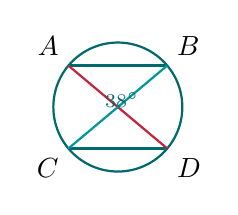
\begin{tikzpicture}[scale=0.78]
      \coordinate (O) at (0,0);
      \draw[thick, color=brandNavy] (O) circle (1.05);
      \coordinate (A) at (140:1.05);
      \coordinate (B) at (40:1.05);
      \coordinate (C) at (220:1.05);
      \coordinate (D) at (-40:1.05);
      \draw[thick, color=brandNavy] (A) -- (B);
      \draw[thick, color=brandNavy] (C) -- (D);
      \draw[thick, color=brandCrimson] (A) -- (D);
      \draw[thick, color=brandBlue] (B) -- (C);
      \node[above left] at (A) {$A$};
      \node[above right] at (B) {$B$};
      \node[below left] at (C) {$C$};
      \node[below right] at (D) {$D$};
      \node[below left, font=\fontsize{7}{7}\selectfont, color=brandNavy] at (0.5,0.4) {$38^\circ$};
    \end{tikzpicture}
  \end{minipage}
\end{khcard}

% =========================================================================
% SECTION 2.4: មុំផ្ចិត និងមុំចារឹកក្នុងរង្វង់
% =========================================================================
\vspace{3pt}
\khsubsection{២.៤}{មុំផ្ចិត និងមុំចារឹកក្នុងរង្វង់}

\begin{khboxorange}
  \textbf{មុំផ្ចិតនៃរង្វង់មួយមានរង្វាស់ស្មើពីរដងមុំចារឹកក្នុងរង្វង់ដែលស្ទាក់ធ្នូតែមួយ ៖} \quad \koreahl{$a = 2b$}
  \par\vspace{1pt}
  \centerline{\begin{tikzpicture}[scale=0.76]
      % Case 1
      \begin{scope}[xshift=0cm]
        \coordinate (O) at (0,0);
        \draw[thick, color=brandNavy] (O) circle (0.95);
        \coordinate (A) at (210:0.95);
        \coordinate (C) at (330:0.95);
        \coordinate (B) at (90:0.95);
        \draw[thick, color=brandCrimson] (O) -- (A) -- (B) -- (C) -- (O);
        \fill[brandNavy] (O) circle (1.5pt);
        \node[below, font=\fontsize{7}{7}\selectfont] at (0,0) {$a$};
        \node[below, font=\fontsize{7}{7}\selectfont] at (0,0.7) {$b$};
        \node[below] at (0,-1.05) {\small\textbf{ផ្ចិតនៅលើជ្រុងមុំ}};
      \end{scope}
      % Case 2
      \begin{scope}[xshift=5.6cm]
        \coordinate (O) at (0,0);
        \draw[thick, color=brandNavy] (O) circle (0.95);
        \coordinate (A) at (220:0.95);
        \coordinate (C) at (320:0.95);
        \coordinate (B) at (85:0.95);
        \draw[thick, color=brandNavy] (A) -- (B) -- (C);
        \draw[thick, color=brandCrimson] (A) -- (O) -- (C);
        \fill[brandNavy] (O) circle (1.5pt);
        \node[above, font=\fontsize{7}{7}\selectfont] at (0,-0.2) {$a$};
        \node[below, font=\fontsize{7}{7}\selectfont] at (0,0.65) {$b$};
        \node[below] at (0,-1.05) {\small\textbf{ផ្ចិតនៅខាងក្នុងមុំ}};
      \end{scope}
      % Case 3
      \begin{scope}[xshift=11.2cm]
        \coordinate (O) at (0,0);
        \draw[thick, color=brandNavy] (O) circle (0.95);
        \coordinate (A) at (200:0.95);
        \coordinate (C) at (260:0.95);
        \coordinate (B) at (60:0.95);
        \draw[thick, color=brandNavy] (A) -- (B) -- (C);
        \draw[thick, color=brandCrimson] (A) -- (O) -- (C);
        \fill[brandNavy] (O) circle (1.5pt);
        \node[left, font=\fontsize{7}{7}\selectfont] at (-0.2,-0.2) {$a$};
        \node[below left, font=\fontsize{7}{7}\selectfont] at (0.4,0.6) {$b$};
        \node[below] at (0,-1.05) {\small\textbf{ផ្ចិតនៅខាងក្រៅមុំ}};
      \end{scope}
    \end{tikzpicture}}
\end{khboxorange}


\begin{khcard}
  \exhead{21} ក្នុងរូបខាងក្រោមនេះ ចូររករង្វាស់មុំ $x$, $y$ និង $a$ ៖
  \par\vspace{1pt}
  \centerline{\begin{tikzpicture}[scale=0.76]
      % Sub-figure (a)
      \begin{scope}[xshift=0cm]
        \coordinate (O) at (0,0);
        \draw[thick, color=brandNavy] (O) circle (0.95);
        \coordinate (A) at (110:0.95);
        \coordinate (B) at (240:0.95);
        \coordinate (C) at (-20:0.95);
        \draw[thick, color=brandNavy] (B) -- (A) -- (C);
        \draw[thick, color=brandCrimson] (B) -- (O) -- (C);
        \fill[brandNavy] (O) circle (1.5pt) node[above right] {$O$};
        \node[above] at (A) {$A$};
        \node[below left] at (B) {$B$};
        \node[right] at (C) {$C$};
        \node[below, font=\fontsize{7}{7}\selectfont] at (-0.15,0.75) {$x$};
        \node[above, font=\fontsize{7}{7}\selectfont, color=brandCrimson] at (0,-0.22) {$76^\circ$};
        \node[below] at (0,-1.15) {\khlabel{ក}};
      \end{scope}
      % Sub-figure (b)
      \begin{scope}[xshift=5.6cm]
        \coordinate (O) at (0,0);
        \draw[thick, color=brandNavy] (O) circle (0.95);
        \coordinate (P) at (90:0.95);
        \coordinate (Q) at (190:0.95);
        \coordinate (R) at (-10:0.95);
        \draw[thick, color=brandNavy] (Q) -- (P) -- (R);
        \draw[thick, color=brandCrimson] (Q) -- (O) -- (R);
        \fill[brandNavy] (O) circle (1.5pt) node[above] {$O$};
        \node[above] at (P) {$P$};
        \node[left] at (Q) {$Q$};
        \node[right] at (R) {$R$};
        \node[below, font=\fontsize{7}{7}\selectfont] at (0,0.7) {$100^\circ$};
        \node[below, font=\fontsize{7}{7}\selectfont, color=brandCrimson] at (0,-0.12) {$y$};
        \node[below] at (0,-1.15) {\khlabel{ខ}};
      \end{scope}
      % Sub-figure (c)
      \begin{scope}[xshift=11.2cm]
        \coordinate (O) at (0,0);
        \draw[thick, color=brandNavy] (O) circle (0.95);
        \coordinate (X) at (80:0.95);
        \coordinate (W) at (170:0.95);
        \coordinate (Y) at (10:0.95);
        \draw[thick, color=brandNavy] (W) -- (X) -- (Y);
        \draw[thick, color=brandCrimson] (W) -- (O) -- (Y);
        \fill[brandNavy] (O) circle (1.5pt) node[below] {$O$};
        \node[above] at (X) {$X$};
        \node[left] at (W) {$W$};
        \node[right] at (Y) {$Y$};
        \node[below, font=\fontsize{7}{7}\selectfont] at (0.1,0.7) {$a$};
        \node[above, font=\fontsize{7}{7}\selectfont, color=brandCrimson] at (0.05,0.12) {$130^\circ$};
        \node[below] at (0,-1.15) {\khlabel{គ}};
      \end{scope}
    \end{tikzpicture}}
  \vspace{1pt}
\end{khcard}


\begin{multicols}{2}
  \noindent
  \begin{minipage}{\linewidth}
    \exhead{22} រង្វង់មួយមានផ្ចិត $O$ ដែល $\angle OBC = 30^\circ$ (ដូចរូប) ។\\
    ចូរគណនារង្វាស់មុំ ៖ \quad $\angle BCO$, $\angle BOC$ និង $\angle BAC$
    \par\vspace{1pt}
    \centerline{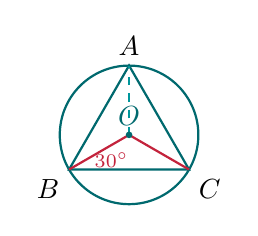
\begin{tikzpicture}[scale=0.80]
        \coordinate (O) at (0,0);
        \draw[thick, color=brandNavy] (O) circle (1.1);
        \coordinate (A) at (90:1.1);
        \coordinate (B) at (210:1.1);
        \coordinate (C) at (330:1.1);
        \draw[thick, color=brandNavy] (A) -- (B) -- (C) -- cycle;
        \draw[thick, color=brandCrimson] (O) -- (B);
        \draw[thick, color=brandCrimson] (O) -- (C);
        \draw[thick, dashed, color=brandTeal] (O) -- (A);
        \fill[brandNavy] (O) circle (1.5pt) node[above] {$O$};
        \node[above] at (A) {$A$};
        \node[below left] at (B) {$B$};
        \node[below right] at (C) {$C$};
        \node[right, font=\fontsize{7}{7}\selectfont, color=brandCrimson] at (-0.7,-0.4) {$30^\circ$};
      \end{tikzpicture}}
  \end{minipage}

  \columnbreak

  \noindent
  \begin{minipage}{\linewidth}
    \exhead{23} រង្វង់មួយមានផ្ចិត $O$ ដែល $\angle OBC = 35^\circ$ ។\\
    ចូរគណនារង្វាស់មុំ ៖ \quad $\angle BCO$, $\angle BOC$ និង $\angle BAC$
    \par\vspace{1pt}
    \centerline{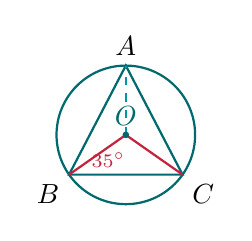
\begin{tikzpicture}[scale=0.80]
        \coordinate (O) at (0,0);
        \draw[thick, color=brandNavy] (O) circle (1.1);
        \coordinate (A) at (90:1.1);
        \coordinate (B) at (215:1.1);
        \coordinate (C) at (325:1.1);
        \draw[thick, color=brandNavy] (A) -- (B) -- (C) -- cycle;
        \draw[thick, color=brandCrimson] (O) -- (B);
        \draw[thick, color=brandCrimson] (O) -- (C);
        \draw[thick, dashed, color=brandTeal] (O) -- (A);
        \fill[brandNavy] (O) circle (1.5pt) node[above] {$O$};
        \node[above] at (A) {$A$};
        \node[below left] at (B) {$B$};
        \node[below right] at (C) {$C$};
        \node[right, font=\fontsize{7}{7}\selectfont, color=brandCrimson] at (-0.7,-0.4) {$35^\circ$};
      \end{tikzpicture}}
  \end{minipage}
\end{multicols}


\begin{multicols}{2}
  \noindent
  \begin{minipage}{\linewidth}
    \exhead{24} រង្វង់មួយមានផ្ចិត $O$ ដែល $\angle ABO = 30^\circ$ និង $\angle ACO = 20^\circ$ ។\\
    ចូរគណនារង្វាស់មុំ ៖ \quad $\angle BAC$ និង $\angle BOC$
    \par\vspace{1pt}
    \centerline{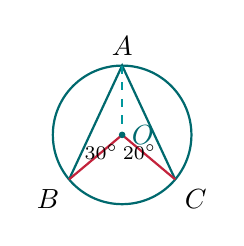
\begin{tikzpicture}[scale=0.80]
        \coordinate (O) at (0,0);
        \draw[thick, color=brandNavy] (O) circle (1.1);
        \coordinate (A) at (90:1.1);
        \coordinate (B) at (220:1.1);
        \coordinate (C) at (-40:1.1);
        \draw[thick, color=brandNavy] (B) -- (A) -- (C);
        \draw[thick, color=brandCrimson] (B) -- (O) -- (C);
        \draw[thick, dashed, color=brandTeal] (A) -- (O);
        \fill[brandNavy] (O) circle (1.5pt) node[right] {$O$};
        \node[above] at (A) {$A$};
        \node[below left] at (B) {$B$};
        \node[below right] at (C) {$C$};
        \node[above right, font=\fontsize{7}{7}\selectfont] at (-0.75,-0.55) {$30^\circ$};
        \node[above left, font=\fontsize{7}{7}\selectfont] at (0.7,-0.55) {$20^\circ$};
      \end{tikzpicture}}
  \end{minipage}

  \columnbreak

  \noindent
  \begin{minipage}{\linewidth}
    \exhead{25} រង្វង់មួយមានផ្ចិត $O$ ដែលមុំផ្ចិត $\angle AOB = 60^\circ$ ។\\
    ចូរគណនារង្វាស់មុំ ៖ \quad $\angle ACB$, $\angle ADB$ និង $\angle AEB$ (ដូចរូបខាងស្ដាំ) ។
    \par\vspace{1pt}
    \centerline{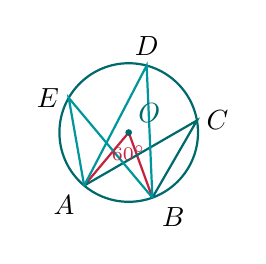
\begin{tikzpicture}[scale=0.80]
        \coordinate (O) at (0,0);
        \draw[thick, color=brandNavy] (O) circle (1.1);
        \coordinate (A) at (230:1.1);
        \coordinate (B) at (290:1.1);
        \coordinate (C) at (10:1.1);
        \coordinate (D) at (75:1.1);
        \coordinate (E) at (150:1.1);
        \draw[thick, color=brandCrimson] (A) -- (O) -- (B);
        \draw[thick, color=brandNavy] (A) -- (C) -- (B);
        \draw[thick, color=brandTeal] (A) -- (D) -- (B);
        \draw[thick, color=brandBlue] (A) -- (E) -- (B);
        \fill[brandNavy] (O) circle (1.5pt) node[above right] {$O$};
        \node[below left] at (A) {$A$};
        \node[below right] at (B) {$B$};
        \node[right] at (C) {$C$};
        \node[above] at (D) {$D$};
        \node[left] at (E) {$E$};
        \node[above, font=\fontsize{7}{7}\selectfont, color=brandCrimson] at (0,-0.6) {$60^\circ$};
      \end{tikzpicture}}
  \end{minipage}
\end{multicols}
\vspace{-0.5cm}
% =========================================================================
% SECTION 3: មុំចារឹកក្នុងកន្លះរង្វង់
% =========================================================================
\khsection{៣}{មុំចារឹកក្នុងកន្លះរង្វង់}

\begin{khboxorange}
	\vspace{-0.3cm}
  \begin{minipage}[c]{0.70\textwidth}
    \raggedright
    \textbf{គ្រប់មុំចារឹកក្នុងកន្លះរង្វង់ជាមុំកែង ៖}{\koreahl{$a = 90^\circ$}}
    \vspace{2pt}
    បើ $AB$ ជាអង្កត់ផ្ចិតនៃរង្វង់ផ្ចិត $O$ ហើយ $C$ ជាចំណុចនៅលើរង្វង់ នោះត្រីកោណ $ABC$ ជាត្រីកោណកែងត្រង់ $C$ ($\angle ACB = 90^\circ$) ។
  \end{minipage}\hfill
  \begin{minipage}[c]{0.28\textwidth}
    \centering
    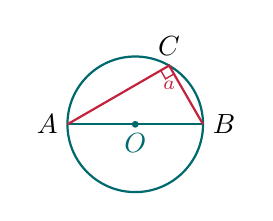
\begin{tikzpicture}[scale=0.82]
      \coordinate (O) at (0,0);
      \draw[thick, color=brandNavy] (O) circle (1.05);
      \coordinate (A) at (-1.05,0);
      \coordinate (B) at (1.05,0);
      \coordinate (C) at (60:1.05);
      \draw[thick, color=brandNavy] (A) -- (B);
      \draw[thick, color=brandCrimson] (A) -- (C) -- (B);
      \fill[brandNavy] (O) circle (1.5pt) node[below] {$O$};
      \node[left] at (A) {$A$};
      \node[right] at (B) {$B$};
      \node[above] at (C) {$C$};
      \draw[color=brandCrimson, line width=0.5pt] ($(C)!0.15cm!(A)$) -- ($($(C)!0.15cm!(A)$)+($(C)!0.15cm!(B)$)-(C)$) -- ($(C)!0.15cm!(B)$);
      \node[below=2pt, font=\fontsize{7.5}{7.5}\selectfont, color=brandCrimson] at (C) {$a$};
    \end{tikzpicture}
  \end{minipage}
\end{khboxorange}
\begin{multicols}{2}
  \noindent
  \begin{minipage}{\linewidth}
    \exhead{26} តាមរូបខាងស្ដាំនេះ $AB$ ជាអង្កត់ផ្ចិតនៃរង្វង់ផ្ចិត $O$ ។\\
    បើ $\angle CAB = 60^\circ$ ចូរគណនារង្វាស់មុំ $a$ និង $b$ ៖
    \par\vspace{1pt}
    \centerline{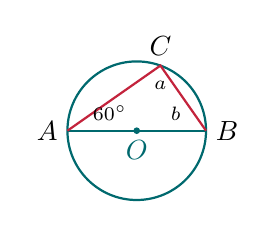
\begin{tikzpicture}[scale=0.80]
        \coordinate (O) at (0,0);
        \draw[thick, color=brandNavy] (O) circle (1.1);
        \coordinate (A) at (-1.1,0);
        \coordinate (B) at (1.1,0);
        \coordinate (C) at (70:1.1);
        \draw[thick, color=brandNavy] (A) -- (B);
        \draw[thick, color=brandCrimson] (A) -- (C) -- (B);
        \fill[brandNavy] (O) circle (1.5pt) node[below] {$O$};
        \node[left] at (A) {$A$};
        \node[right] at (B) {$B$};
        \node[above] at (C) {$C$};
        \node[below=2pt, font=\fontsize{7}{7}\selectfont] at (C) {$a$};
        \node[above right, font=\fontsize{7}{7}\selectfont] at (-0.85,0) {$60^\circ$};
        \node[above left, font=\fontsize{7}{7}\selectfont] at (0.85,0) {$b$};
      \end{tikzpicture}}
  \end{minipage}

  \columnbreak

  \noindent
  \begin{minipage}{\linewidth}
    \exhead{27} តាមរូបខាងស្ដាំនេះ $AB$ ជាអង្កត់ផ្ចិតនៃរង្វង់ផ្ចិត $O$ ។\\
    បើ $\angle CAB = 45^\circ$ ចូរគណនារង្វាស់មុំ $a$ និង $b$ ៖
    \par\vspace{1pt}
    \centerline{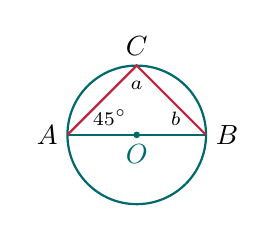
\begin{tikzpicture}[scale=0.80]
        \coordinate (O) at (0,0);
        \draw[thick, color=brandNavy] (O) circle (1.1);
        \coordinate (A) at (-1.1,0);
        \coordinate (B) at (1.1,0);
        \coordinate (C) at (90:1.1);
        \draw[thick, color=brandNavy] (A) -- (B);
        \draw[thick, color=brandCrimson] (A) -- (C) -- (B);
        \fill[brandNavy] (O) circle (1.5pt) node[below] {$O$};
        \node[left] at (A) {$A$};
        \node[right] at (B) {$B$};
        \node[above] at (C) {$C$};
        \node[below=2pt, font=\fontsize{7}{7}\selectfont] at (C) {$a$};
        \node[above right, font=\fontsize{7}{7}\selectfont] at (-0.85,0) {$45^\circ$};
        \node[above left, font=\fontsize{7}{7}\selectfont] at (0.85,0) {$b$};
      \end{tikzpicture}}
  \end{minipage}
\end{multicols}


\begin{multicols}{2}
  \noindent
  \begin{minipage}{\linewidth}
    \exhead{28} រង្វង់មួយមានផ្ចិត $O$ និងអង្កត់ផ្ចិត $AB$ ។\\
    បើ $\angle CAD = 21^\circ$ ចូរគណនារង្វាស់មុំ $a$ និង $b$ (ដូចរូប) ៖
    \par\vspace{1pt}
    \centerline{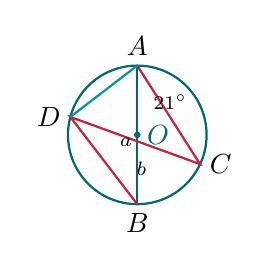
\begin{tikzpicture}[scale=0.80]
        \coordinate (O) at (0,0);
        \draw[thick, color=brandNavy] (O) circle (1.1);
        \coordinate (A) at (90:1.1);
        \coordinate (B) at (-90:1.1);
        \coordinate (C) at (-25:1.1);
        \coordinate (D) at (165:1.1);
        \draw[thick, color=brandNavy] (A) -- (B);
        \draw[thick, color=brandCrimson] (A) -- (C) -- (D) -- (B);
        \draw[thick, color=brandBlue] (A) -- (D);
        \fill[brandNavy] (O) circle (1.5pt) node[right] {$O$};
        \node[above] at (A) {$A$};
        \node[below] at (B) {$B$};
        \node[right] at (C) {$C$};
        \node[left] at (D) {$D$};
        \node[below right, font=\fontsize{7}{7}\selectfont] at (0.1,0.8) {$21^\circ$};
        \node[below, font=\fontsize{7}{7}\selectfont] at (-0.18,0.1) {$a$};
        \node[above left, font=\fontsize{7}{7}\selectfont] at (0.3,-0.8) {$b$};
      \end{tikzpicture}}
  \end{minipage}

  \columnbreak

  \noindent
  \begin{minipage}{\linewidth}
    \exhead{29} តាមរូបខាងស្ដាំ គេមានរង្វង់ផ្ចិត $O$ អង្កត់ផ្ចិត $AB$ និង $PT$ ជាបន្ទាត់ប៉ះរង្វង់ត្រង់ $T$ ។ បើ $\angle TAP = 35^\circ$ ចូរគណនា ៖\\
    \khlabel{ក} $\angle ATB$ \qquad \khlabel{ខ} $\angle APT$ \qquad \khlabel{គ} $\angle BTP$
    \par\vspace{1pt}
    \centerline{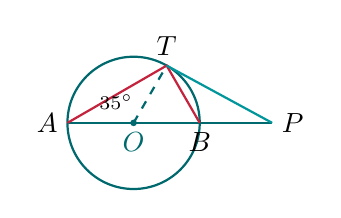
\begin{tikzpicture}[scale=0.80]
        \coordinate (O) at (0,0);
        \draw[thick, color=brandNavy] (O) circle (1.05);
        \coordinate (A) at (-1.05,0);
        \coordinate (B) at (1.05,0);
        \coordinate (T) at (60:1.05);
        \coordinate (P) at (2.2,0);
        \draw[thick, color=brandNavy] (A) -- (P);
        \draw[thick, color=brandCrimson] (A) -- (T) -- (B);
        \draw[thick, color=brandTeal] (T) -- (P);
        \draw[thick, dashed, color=brandNavy] (O) -- (T);
        \fill[brandNavy] (O) circle (1.5pt) node[below] {$O$};
        \node[left] at (A) {$A$};
        \node[below] at (B) {$B$};
        \node[above] at (T) {$T$};
        \node[right] at (P) {$P$};
        \node[above right, font=\fontsize{7}{7}\selectfont] at (-0.7,0.05) {$35^\circ$};
      \end{tikzpicture}}
  \end{minipage}
\end{multicols}

\begin{multicols}{2}
  \noindent
  \begin{minipage}{\linewidth}
    \exhead{30} តាមរូបខាងស្ដាំនេះ គេមានរង្វង់ផ្ចិត $O$ និងអង្កត់ផ្ចិត $AC$ ហើយ $AD = DC$ ។ ចូរគណនារង្វាស់មុំ $x$, $y$ និង $z$ ៖
    \par\vspace{1pt}
    \centerline{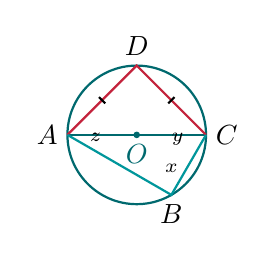
\begin{tikzpicture}[scale=0.80]
        \coordinate (O) at (0,0);
        \draw[thick, color=brandNavy] (O) circle (1.1);
        \coordinate (A) at (-1.1,0);
        \coordinate (C) at (1.1,0);
        \coordinate (D) at (90:1.1);
        \coordinate (B) at (-60:1.1);
        \draw[thick, color=brandNavy] (A) -- (C);
        \draw[thick, color=brandCrimson] (A) -- (D) -- (C);
        \draw[thick, color=brandBlue] (A) -- (B) -- (C);
        \fill[brandNavy] (O) circle (1.5pt) node[below] {$O$};
        \node[left] at (A) {$A$};
        \node[right] at (C) {$C$};
        \node[above] at (D) {$D$};
        \node[below] at (B) {$B$};
        \node[below right, font=\fontsize{7}{7}\selectfont] at (-0.9,0.18) {$z$};
        \node[below left, font=\fontsize{7}{7}\selectfont] at (0.9,0.18) {$y$};
        \node[above, font=\fontsize{7}{7}\selectfont] at (0.55,-0.75) {$x$};
        \draw[thick] ($(A)!0.5!(D)$) ++(-0.05,0.05) -- ++(0.1,-0.1);
        \draw[thick] ($(C)!0.5!(D)$) ++(-0.05,-0.05) -- ++(0.1,0.1);
      \end{tikzpicture}}
  \end{minipage}

  \columnbreak

  \noindent
  \begin{minipage}{\linewidth}
    \exhead{31} ក្នុងរង្វង់ផ្ចិត $O$ មាន $AC$ ជាអង្កត់ផ្ចិត ។ គេបន្លាយអង្កត់ធ្នូ $BA$ និង $CD$ ឱ្យជួបគ្នាត្រង់ $T$ ហើយ $AT = AC$ និង $\angle ATD = 20^\circ$ ។\\
    ចូរគណនារង្វាស់មុំ ៖ \quad \khlabel{ក} $\angle ADB$ \qquad \khlabel{ខ} $\angle BOC$ \qquad \khlabel{គ} $\angle BDC$
    \par\vspace{1pt}
    \centerline{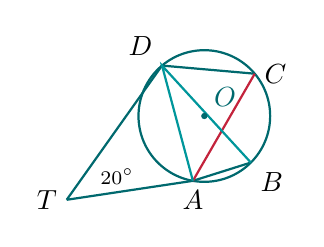
\begin{tikzpicture}[scale=0.76]
        \coordinate (O) at (0,0);
        \draw[thick, color=brandNavy] (O) circle (1.1);
        \coordinate (C) at (40:1.1);
        \coordinate (B) at (-45:1.1);
        \coordinate (A) at (-100:1.1);
        \coordinate (D) at (130:1.1);
        \coordinate (T) at (-2.3,-1.4);
        \draw[thick, color=brandNavy] (B) -- (A) -- (T);
        \draw[thick, color=brandNavy] (C) -- (D) -- (T);
        \draw[thick, color=brandCrimson] (A) -- (C);
        \draw[thick, color=brandBlue] (A) -- (D) -- (B);
        \fill[brandNavy] (O) circle (1.5pt) node[above right] {$O$};
        \node[right] at (C) {$C$};
        \node[below right] at (B) {$B$};
        \node[below] at (A) {$A$};
        \node[above left] at (D) {$D$};
        \node[left] at (T) {$T$};
        \node[above right, font=\fontsize{7}{7}\selectfont] at (-1.9,-1.3) {$20^\circ$};
      \end{tikzpicture}}
  \end{minipage}
\end{multicols}

% =========================================================================
% SECTION 4: មុំឈមនៃចតុកោណចារឹកក្នុងរង្វង់
% =========================================================================
\vspace{-0.5cm}
\khsection{៤}{មុំឈមនៃចតុកោណចារឹកក្នុងរង្វង់}

\begin{khcard}
  \begin{minipage}[c]{0.70\textwidth}
    \textbf{៤.១ និយមន័យ ៖} ចតុកោណដែលមានកំពូលទាំងបួនស្ថិតនៅលើរង្វង់តែមួយ ហៅថាចតុកោណចារឹកក្នុងរង្វង់ ។ រង្វង់នោះហៅថា រង្វង់ចារឹកក្រៅចតុកោណ ។\\
    \textbf{៤.២ លក្ខណៈមុំឈម ៖} មុំឈមក្នុងចតុកោណចារឹកក្នុងរង្វង់មួយជាមុំបន្ថែមគ្នា ៖
    \begin{equation*}
      \koreahl{$a + c = 180^\circ$} \qquad \text{និង} \qquad \koreahl{$b + d = 180^\circ$}
    \end{equation*}
  \end{minipage}\hfill
  \begin{minipage}[c]{0.28\textwidth}
    \centering
    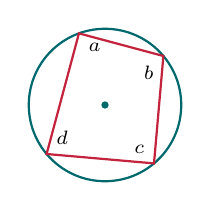
\begin{tikzpicture}[scale=0.88]
      \coordinate (O) at (0,0);
      \draw[thick, color=brandNavy] (O) circle (1.1);
      \coordinate (A) at (110:1.1);
      \coordinate (B) at (40:1.1);
      \coordinate (C) at (-50:1.1);
      \coordinate (D) at (220:1.1);
      \draw[thick, color=brandCrimson] (A) -- (B) -- (C) -- (D) -- cycle;
      \fill[brandNavy] (O) circle (1.5pt);
      \node[below right, font=\fontsize{7.5}{7.5}\selectfont] at (A) {$a$};
      \node[below left, font=\fontsize{7.5}{7.5}\selectfont] at (B) {$b$};
      \node[above left, font=\fontsize{7.5}{7.5}\selectfont] at (C) {$c$};
      \node[above right, font=\fontsize{7.5}{7.5}\selectfont] at (D) {$d$};
    \end{tikzpicture}
  \end{minipage}
\end{khcard}

\begin{multicols}{2}
  \noindent
  \begin{minipage}{\linewidth}
    \exhead{32} គេឱ្យចតុកោណ $ABCD$ ចារឹកក្នុងរង្វង់ផ្ចិត $O$ ដូចរូបខាងស្ដាំ ។ បើ $\angle DAB = 80^\circ$ និង $\angle ABC = 70^\circ$ ចូរគណនារង្វាស់មុំ $x$ និង $y$ ៖
    \begin{center}
      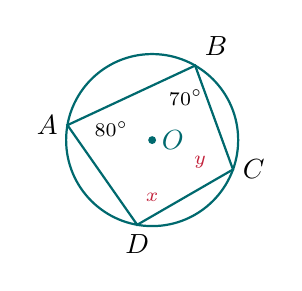
\begin{tikzpicture}[scale=0.95]
        \coordinate (O) at (0,0);
        \draw[thick, color=brandNavy] (O) circle (1.15);
        \coordinate (A) at (170:1.15);
        \coordinate (B) at (60:1.15);
        \coordinate (C) at (-20:1.15);
        \coordinate (D) at (260:1.15);
        \draw[thick, color=brandNavy] (A) -- (B) -- (C) -- (D) -- cycle;
        \fill[brandNavy] (O) circle (1.5pt) node[right] {$O$};
        \node[left] at (A) {$A$};
        \node[above right] at (B) {$B$};
        \node[right] at (C) {$C$};
        \node[below] at (D) {$D$};
        \node[right, font=\fontsize{7.5}{7.5}\selectfont] at (-0.9,0.15) {$80^\circ$};
        \node[below, font=\fontsize{7.5}{7.5}\selectfont] at (0.45,0.8) {$70^\circ$};
        \node[above, font=\fontsize{7.5}{7.5}\selectfont, color=brandCrimson] at (0,-0.95) {$x$};
        \node[left, font=\fontsize{7.5}{7.5}\selectfont, color=brandCrimson] at (0.85,-0.3) {$y$};
      \end{tikzpicture}
    \end{center}
  \end{minipage}

  \columnbreak

  \noindent
  \begin{minipage}{\linewidth}
    \exhead{33} គេឱ្យចតុកោណ $ABCD$ ចារឹកក្នុងរង្វង់ផ្ចិត $O$ ។ បើ $\angle DAB = 85^\circ$ និង $\angle ABC = 65^\circ$ ចូរគណនារង្វាស់មុំឈមនៃកំពូលទាំងពីរនេះ ៖
    \begin{center}
      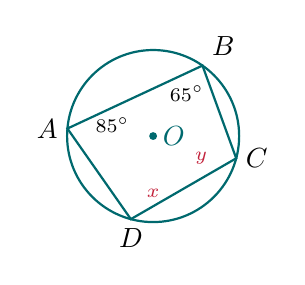
\begin{tikzpicture}[scale=0.95]
        \coordinate (O) at (0,0);
        \draw[thick, color=brandNavy] (O) circle (1.15);
        \coordinate (A) at (175:1.15);
        \coordinate (B) at (55:1.15);
        \coordinate (C) at (-15:1.15);
        \coordinate (D) at (255:1.15);
        \draw[thick, color=brandNavy] (A) -- (B) -- (C) -- (D) -- cycle;
        \fill[brandNavy] (O) circle (1.5pt) node[right] {$O$};
        \node[left] at (A) {$A$};
        \node[above right] at (B) {$B$};
        \node[right] at (C) {$C$};
        \node[below] at (D) {$D$};
        \node[right, font=\fontsize{7.5}{7.5}\selectfont] at (-0.9,0.15) {$85^\circ$};
        \node[below, font=\fontsize{7.5}{7.5}\selectfont] at (0.45,0.8) {$65^\circ$};
        \node[above, font=\fontsize{7.5}{7.5}\selectfont, color=brandCrimson] at (0,-0.95) {$x$};
        \node[left, font=\fontsize{7.5}{7.5}\selectfont, color=brandCrimson] at (0.85,-0.3) {$y$};
      \end{tikzpicture}
    \end{center}
  \end{minipage}
\end{multicols}

\begin{multicols}{2}
  \noindent
  \begin{minipage}{\linewidth}
    \exhead{34} តាមរូបខាងស្ដាំនេះ ចូររករង្វាស់មុំ $a$ និង $b$ ៖
    \begin{center}
      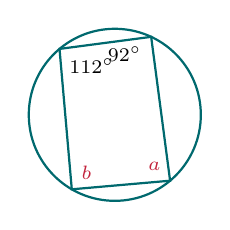
\begin{tikzpicture}[scale=0.95]
        \coordinate (O) at (0,0);
        \draw[thick, color=brandNavy] (O) circle (1.15);
        \coordinate (P1) at (130:1.15);
        \coordinate (P2) at (65:1.15);
        \coordinate (P3) at (-50:1.15);
        \coordinate (P4) at (240:1.15);
        \draw[thick, color=brandNavy] (P1) -- (P2) -- (P3) -- (P4) -- cycle;
        \node[below right, font=\fontsize{7.5}{7.5}\selectfont] at (P1) {$112^\circ$};
        \node[below left, font=\fontsize{7.5}{7.5}\selectfont] at (P2) {$92^\circ$};
        \node[above left, font=\fontsize{7.5}{7.5}\selectfont, color=brandCrimson] at (P3) {$a$};
        \node[above right, font=\fontsize{7.5}{7.5}\selectfont, color=brandCrimson] at (P4) {$b$};
      \end{tikzpicture}
    \end{center}
  \end{minipage}

  \columnbreak

  \noindent
  \begin{minipage}{\linewidth}
    \exhead{35} តាមរូបខាងស្ដាំនេះ ចូររករង្វាស់មុំ $a$ និង $b$ ៖
    \begin{center}
      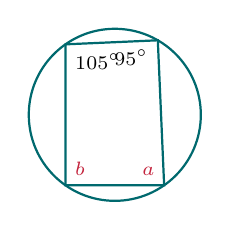
\begin{tikzpicture}[scale=0.95]
        \coordinate (O) at (0,0);
        \draw[thick, color=brandNavy] (O) circle (1.15);
        \coordinate (P1) at (125:1.15);
        \coordinate (P2) at (60:1.15);
        \coordinate (P3) at (-55:1.15);
        \coordinate (P4) at (235:1.15);
        \draw[thick, color=brandNavy] (P1) -- (P2) -- (P3) -- (P4) -- cycle;
        \node[below right, font=\fontsize{7.5}{7.5}\selectfont] at (P1) {$105^\circ$};
        \node[below left, font=\fontsize{7.5}{7.5}\selectfont] at (P2) {$95^\circ$};
        \node[above left, font=\fontsize{7.5}{7.5}\selectfont, color=brandCrimson] at (P3) {$a$};
        \node[above right, font=\fontsize{7.5}{7.5}\selectfont, color=brandCrimson] at (P4) {$b$};
      \end{tikzpicture}
    \end{center}
  \end{minipage}
\end{multicols}

% =========================================================================
% SECTION 5: មុំក្រៅនៃចតុកោណចារឹកក្នុងរង្វង់
% =========================================================================
\vspace{-0.5cm}
\khsection{៥}{មុំក្រៅនៃចតុកោណចារឹកក្នុងរង្វង់}

\begin{khboxorange}
  \begin{minipage}[c]{0.75\textwidth}
    \textbf{មុំក្រៅនៃចតុកោណចារឹកក្នុងរង្វង់មានរង្វាស់ស្មើនឹងមុំឈមវាចារឹកក្នុងចតុកោណនោះ ៖} \koreahl{$p = q$}\text{និង}\koreahl{$r = s$}
  \end{minipage}\hfill
  \begin{minipage}[c]{0.2\textwidth}
    \centering
    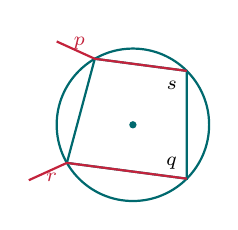
\begin{tikzpicture}[scale=0.88]
      \coordinate (O) at (0,0);
      \draw[thick, color=brandNavy] (O) circle (1.1);
      \coordinate (A) at (120:1.1);
      \coordinate (B) at (45:1.1);
      \coordinate (C) at (-45:1.1);
      \coordinate (D) at (210:1.1);
      \draw[thick, color=brandNavy] (A) -- (B) -- (C) -- (D) -- cycle;
      \draw[thick, color=brandCrimson] (B) -- (A) -- ++(-0.55,0.25);
      \draw[thick, color=brandCrimson] (C) -- (D) -- ++(-0.55,-0.25);
      \fill[brandNavy] (O) circle (1.5pt);
      \node[above left, font=\fontsize{7.5}{7.5}\selectfont, color=brandCrimson] at (A) {$p$};
      \node[below left, font=\fontsize{7.5}{7.5}\selectfont, color=brandCrimson] at (D) {$r$};
      \node[below left, font=\fontsize{7.5}{7.5}\selectfont] at (B) {$s$};
      \node[above left, font=\fontsize{7.5}{7.5}\selectfont] at (C) {$q$};
    \end{tikzpicture}
  \end{minipage}
\end{khboxorange}

\vspace{3pt}
\Needspace*{6.8cm}
\begin{multicols}{2}
  \noindent
  \begin{minipage}{\linewidth}
    \exhead{36} គេមានរង្វង់ផ្ចិត $O$ និង $ABC$ ជាត្រីកោណ ។ បើរង្វង់កាត់ $BC$ ត្រង់ $C$ និង $AE$ ត្រង់ $D$ ។\\
    បើ $\angle B = 40^\circ$ និង $\angle A = 110^\circ$ ចូរគណនារង្វាស់មុំ $x, y$ និង $z$ ៖
    \begin{center}
      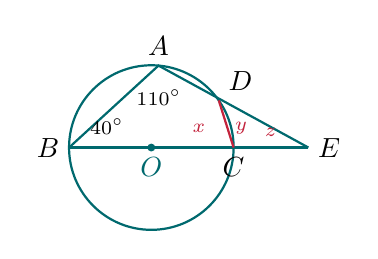
\begin{tikzpicture}[scale=0.95]
        \coordinate (O) at (0,0);
        \draw[thick, color=brandNavy] (O) circle (1.1);
        \coordinate (B) at (-1.1,0);
        \coordinate (C) at (1.1,0);
        \coordinate (A) at (85:1.1);
        \coordinate (D) at (35:1.1);
        \coordinate (E) at (2.1,0);
        \draw[thick, color=brandNavy] (B) -- (E);
        \draw[thick, color=brandNavy] (B) -- (A) -- (E);
        \draw[thick, color=brandCrimson] (C) -- (D);
        \fill[brandNavy] (O) circle (1.5pt) node[below] {$O$};
        \node[left] at (B) {$B$};
        \node[below] at (C) {$C$};
        \node[above] at (A) {$A$};
        \node[above right] at (D) {$D$};
        \node[right] at (E) {$E$};
        \node[above right, font=\fontsize{7.5}{7.5}\selectfont] at (-0.95,0.05) {$40^\circ$};
        \node[below, font=\fontsize{7.5}{7.5}\selectfont] at (0.1,0.9) {$110^\circ$};
        \node[below left, font=\fontsize{7.5}{7.5}\selectfont, color=brandCrimson] at (0.85,0.45) {$x$};
        \node[above, font=\fontsize{7.5}{7.5}\selectfont, color=brandCrimson] at (1.2,0.05) {$y$};
        \node[above left, font=\fontsize{7.5}{7.5}\selectfont, color=brandCrimson] at (1.8,0.02) {$z$};
      \end{tikzpicture}
    \end{center}
  \end{minipage}

  \columnbreak

  \noindent
  \begin{minipage}{\linewidth}
    \exhead{37} $ABCD$ ជាចតុកោណចារឹកក្នុងរង្វង់ដែលមាន $AD = AB$ ហើយ $AD$ បន្លាយទៅ $E$ ។\\
    បើ $\angle CDE = 70^\circ$ និង $\angle CDB = 72^\circ$ ចូរគណនា ៖\\
    \khlabel{ក} $\angle BAD$ \qquad \khlabel{ខ} $\angle BCD$
    \begin{center}
      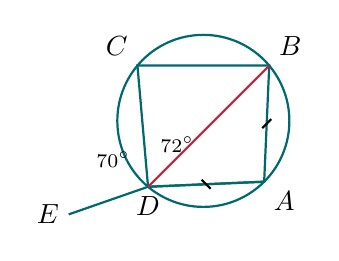
\begin{tikzpicture}[scale=0.95]
        \coordinate (O) at (0,0);
        \draw[thick, color=brandNavy] (O) circle (1.15);
        \coordinate (A) at (-45:1.15);
        \coordinate (B) at (40:1.15);
        \coordinate (C) at (140:1.15);
        \coordinate (D) at (230:1.15);
        \coordinate (E) at (-1.8,-1.25);
        \draw[thick, color=brandNavy] (A) -- (B) -- (C) -- (D) -- cycle;
        \draw[thick, color=brandNavy] (A) -- (D) -- (E);
        \draw[thick, color=brandCrimson] (D) -- (B);
        \node[below right] at (A) {$A$};
        \node[above right] at (B) {$B$};
        \node[above left] at (C) {$C$};
        \node[below] at (D) {$D$};
        \node[left] at (E) {$E$};
        \node[above left, font=\fontsize{7.5}{7.5}\selectfont] at (-0.85,-0.75) {$70^\circ$};
        \node[above, font=\fontsize{7.5}{7.5}\selectfont] at (-0.35,-0.55) {$72^\circ$};
        \draw[thick] ($(A)!0.5!(B)$) ++(-0.06,-0.06) -- ++(0.12,0.12);
        \draw[thick] ($(A)!0.5!(D)$) ++(-0.06,0.06) -- ++(0.12,-0.12);
      \end{tikzpicture}
    \end{center}
  \end{minipage}
\end{multicols}

\begin{multicols}{2}
  \noindent
  \begin{minipage}{\linewidth}
    \exhead{38} គេមានចតុកោណ $ABDC$ និង $CDFE$ ជាចតុកោណចារឹកក្នុងរង្វង់រៀងគ្នា (ដូចរូប) ។\\
    បើ $\angle A = 85^\circ$ ចូរគណនារង្វាស់មុំ $a$ ៖
    \begin{center}
      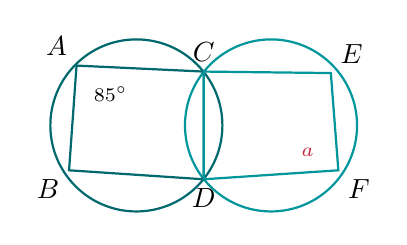
\begin{tikzpicture}[scale=0.95]
        \draw[thick, color=brandNavy] (-0.9,0) circle (1.15);
        \draw[thick, color=brandTeal] (0.9,0) circle (1.15);
        \coordinate (A) at (-1.7,0.8);
        \coordinate (B) at (-1.8,-0.6);
        \coordinate (C) at (0,0.72);
        \coordinate (D) at (0,-0.72);
        \coordinate (E) at (1.7,0.7);
        \coordinate (F) at (1.8,-0.6);
        \draw[thick, color=brandNavy] (A) -- (B) -- (D) -- (C) -- cycle;
        \draw[thick, color=brandTeal] (C) -- (D) -- (F) -- (E) -- cycle;
        \node[above left] at (A) {$A$};
        \node[below left] at (B) {$B$};
        \node[above] at (C) {$C$};
        \node[below] at (D) {$D$};
        \node[above right] at (E) {$E$};
        \node[below right] at (F) {$F$};
        \node[below right, font=\fontsize{7.5}{7.5}\selectfont] at (-1.6,0.65) {$85^\circ$};
        \node[above left, font=\fontsize{7.5}{7.5}\selectfont, color=brandCrimson] at (1.6,-0.55) {$a$};
      \end{tikzpicture}
    \end{center}
  \end{minipage}

  \columnbreak

  \noindent
  \begin{minipage}{\linewidth}
    \exhead{39} $EFGH$ ជាចតុកោណចារឹកក្នុងរង្វង់ផ្ចិត $O$ ដែលមាន $EH \parallel FG$ ហើយ $DG$ ជាអង្កត់ផ្ចិត ។\\
    គេឱ្យ $\angle DOH = 82^\circ$ និង $\angle DGE = 17^\circ$ ។ ចូរគណនា ៖\\
    \khlabel{ក} $\angle HEG$ \qquad \khlabel{ខ} $\angle HGF$ \qquad \khlabel{គ} $\angle FEG$
    \begin{center}
      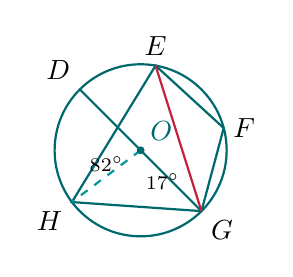
\begin{tikzpicture}[scale=0.95]
        \coordinate (O) at (0,0);
        \draw[thick, color=brandNavy] (O) circle (1.15);
        \coordinate (D) at (135:1.15);
        \coordinate (G) at (-45:1.15);
        \coordinate (E) at (80:1.15);
        \coordinate (F) at (15:1.15);
        \coordinate (H) at (217:1.15);
        \draw[thick, color=brandNavy] (D) -- (G);
        \draw[thick, color=brandNavy] (E) -- (F) -- (G) -- (H) -- cycle;
        \draw[thick, color=brandCrimson] (E) -- (G);
        \draw[thick, dashed, color=brandTeal] (O) -- (H);
        \fill[brandNavy] (O) circle (1.5pt) node[above right] {$O$};
        \node[above left] at (D) {$D$};
        \node[above] at (E) {$E$};
        \node[right] at (F) {$F$};
        \node[below right] at (G) {$G$};
        \node[below left] at (H) {$H$};
        \node[below left, font=\fontsize{7.5}{7.5}\selectfont] at (-0.1,0.05) {$82^\circ$};
        \node[above left, font=\fontsize{7.5}{7.5}\selectfont] at (0.65,-0.65) {$17^\circ$};
      \end{tikzpicture}
    \end{center}
  \end{minipage}
\end{multicols}

\begin{multicols}{2}
  \noindent
  \begin{minipage}{\linewidth}
    \exhead{40} គេមានចតុកោណ $ABCD$ ចារឹកក្នុងរង្វង់ដែលមាន $AB = BC$ ។ គេបន្លាយ $CD$ ដល់ $E$ ដែលមាន $\angle ACE = 27^\circ$ និង $\angle ADE = 76^\circ$ ។\\
    ចូរគណនា ៖ \quad \khlabel{ក} $\angle ACB$ \qquad \khlabel{ខ} $\angle BAD$
    \begin{center}
      \begin{tikzpicture}[scale=0.95]
        \coordinate (O) at (0,0);
        \draw[thick, color=brandNavy] (O) circle (1.15);
        \coordinate (B) at (110:1.15);
        \coordinate (A) at (30:1.15);
        \coordinate (C) at (210:1.15);
        \coordinate (D) at (-40:1.15);
        \coordinate (E) at (1.7,-1.15);
        \draw[thick, color=brandNavy] (A) -- (B) -- (C) -- (D) -- cycle;
        \draw[thick, color=brandNavy] (C) -- (D) -- (E);
        \draw[thick, color=brandCrimson] (A) -- (C);
        \node[above] at (B) {$B$};
        \node[right] at (A) {$A$};
        \node[below left] at (C) {$C$};
        \node[below] at (D) {$D$};
        \node[right] at (E) {$E$};
        \node[above right, font=\fontsize{7.5}{7.5}\selectfont] at (-0.65,-0.65) {$27^\circ$};
        \node[above, font=\fontsize{7.5}{7.5}\selectfont] at (1.05,-0.85) {$76^\circ$};
        \draw[thick] ($(A)!0.5!(B)$) ++(-0.06,0.06) -- ++(0.12,-0.12);
        \draw[thick] ($(B)!0.5!(C)$) ++(-0.06,0.06) -- ++(0.12,-0.12);
      \end{tikzpicture}
    \end{center}
  \end{minipage}

  \columnbreak

  \noindent
  \begin{minipage}{\linewidth}
    \exhead{41} គេមាន $ABCD$ ជាចតុកោណចារឹកក្នុងរង្វង់ដែលមាន $AB = BC$ និង $\angle ACE = 25^\circ$ ។ គេបន្លាយ $CD$ ដល់ $E$ និង $\angle ADE = 80^\circ$ ។\\
    ចូរគណនារង្វាស់មុំ ៖ \quad \khlabel{ក} $\angle ABC$ \qquad \khlabel{ខ} $\angle BAD$
    \begin{center}
      \begin{tikzpicture}[scale=0.95]
        \coordinate (O) at (0,0);
        \draw[thick, color=brandNavy] (O) circle (1.15);
        \coordinate (B) at (115:1.15);
        \coordinate (A) at (35:1.15);
        \coordinate (C) at (215:1.15);
        \coordinate (D) at (-35:1.15);
        \coordinate (E) at (1.75,-1.15);
        \draw[thick, color=brandNavy] (A) -- (B) -- (C) -- (D) -- cycle;
        \draw[thick, color=brandNavy] (C) -- (D) -- (E);
        \draw[thick, color=brandTeal] (A) -- (C);
        \node[above] at (B) {$B$};
        \node[right] at (A) {$A$};
        \node[below left] at (C) {$C$};
        \node[below] at (D) {$D$};
        \node[right] at (E) {$E$};
        \node[above right, font=\fontsize{7.5}{7.5}\selectfont] at (-0.65,-0.65) {$25^\circ$};
        \node[above, font=\fontsize{7.5}{7.5}\selectfont] at (1.05,-0.85) {$80^\circ$};
        \draw[thick] ($(A)!0.5!(B)$) ++(-0.06,0.06) -- ++(0.12,-0.12);
        \draw[thick] ($(B)!0.5!(C)$) ++(-0.06,0.06) -- ++(0.12,-0.12);
      \end{tikzpicture}
    \end{center}
  \end{minipage}
\end{multicols}

% =========================================================================
% SECTION 6: មុំដែលមានកំពូលមិននៅលើរង្វង់
% =========================================================================
\vspace{-0.5cm}
\khsection{៦}{មុំដែលមានកំពូលមិននៅលើរង្វង់}
\khsubsection{៦.១}{មុំក្នុងរង្វង់}

\begin{khboxorange}
  \begin{minipage}[c]{0.70\textwidth}
    \textbf{មុំក្នុងរង្វង់ជាមុំដែលមានកំពូលនៅក្នុងរង្វង់ ។}\\
    \textbf{មុំក្នុងរង្វង់មានរង្វាស់ស្មើនឹងកន្លះផលបូករង្វាស់ធ្នូស្ទាក់ដោយជ្រុងនៃមុំ ៖} \koreahl{$\angle SPQ = \frac{\wideparen{SQ} + \wideparen{RT}}{2}$}
  \end{minipage}\hfill
  \begin{minipage}[c]{0.28\textwidth}
    \centering
    \begin{tikzpicture}[scale=0.88]
      \coordinate (O) at (0,0);
      \draw[thick, color=brandNavy] (O) circle (1.1);
      \coordinate (S) at (125:1.1);
      \coordinate (T) at (-35:1.1);
      \coordinate (R) at (30:1.1);
      \coordinate (Q) at (235:1.1);
      \draw[thick, color=brandNavy] (S) -- (T);
      \draw[thick, color=brandNavy] (Q) -- (R);
      \coordinate (P) at (intersection of S--T and Q--R);
      \fill[brandNavy] (O) circle (1.5pt) node[left] {$O$};
      \node[above left] at (S) {$S$};
      \node[below right] at (T) {$T$};
      \node[above right] at (R) {$R$};
      \node[below left] at (Q) {$Q$};
      \node[above] at (P) {$P$};
    \end{tikzpicture}
  \end{minipage}
\end{khboxorange}
\begin{multicols}{2}
  \noindent
  \begin{minipage}{\linewidth}
    \exhead{42} ក្នុងរូបខាងស្ដាំនេះ គេឱ្យ $\wideparen{SQ} = 112^\circ$ និង $\wideparen{RT} = 38^\circ$ ។\\
    ចូរគណនារង្វាស់មុំ $\angle SPQ$ ៖
    \begin{center}
      \begin{tikzpicture}[scale=0.95]
        \coordinate (O) at (0,0);
        \draw[thick, color=brandNavy] (O) circle (1.15);
        \coordinate (S) at (125:1.15);
        \coordinate (T) at (-35:1.15);
        \coordinate (R) at (25:1.15);
        \coordinate (Q) at (240:1.15);
        \draw[thick, color=brandNavy] (S) -- (T);
        \draw[thick, color=brandNavy] (Q) -- (R);
        \coordinate (P) at (intersection of S--T and Q--R);
        \fill[brandNavy] (O) circle (1.5pt) node[left] {$O$};
        \node[above left] at (S) {$S$};
        \node[below right] at (T) {$T$};
        \node[above right] at (R) {$R$};
        \node[below left] at (Q) {$Q$};
        \node[above] at (P) {$P$};
        \node[left, font=\fontsize{7.5}{7.5}\selectfont, color=brandCrimson] at (-1.2,-0.1) {$112^\circ$};
        \node[right, font=\fontsize{7.5}{7.5}\selectfont, color=brandBlue] at (1.2,0) {$38^\circ$};
      \end{tikzpicture}
    \end{center}
  \end{minipage}

  \columnbreak

  \noindent
  \begin{minipage}{\linewidth}
    \exhead{43} ក្នុងរូបខាងស្ដាំនេះ គេឱ្យ $\wideparen{SQ} = 120^\circ$ និង $\wideparen{RT} = 40^\circ$ ។\\
    ចូរគណនារង្វាស់មុំ $\angle SPQ$ ៖
    \begin{center}
      \begin{tikzpicture}[scale=0.95]
        \coordinate (O) at (0,0);
        \draw[thick, color=brandNavy] (O) circle (1.15);
        \coordinate (S) at (130:1.15);
        \coordinate (T) at (-30:1.15);
        \coordinate (R) at (30:1.15);
        \coordinate (Q) at (230:1.15);
        \draw[thick, color=brandNavy] (S) -- (T);
        \draw[thick, color=brandNavy] (Q) -- (R);
        \coordinate (P) at (intersection of S--T and Q--R);
        \fill[brandNavy] (O) circle (1.5pt) node[left] {$O$};
        \node[above left] at (S) {$S$};
        \node[below right] at (T) {$T$};
        \node[above right] at (R) {$R$};
        \node[below left] at (Q) {$Q$};
        \node[above] at (P) {$P$};
        \node[left, font=\fontsize{7.5}{7.5}\selectfont, color=brandCrimson] at (-1.2,-0.1) {$120^\circ$};
        \node[right, font=\fontsize{7.5}{7.5}\selectfont, color=brandBlue] at (1.2,0) {$40^\circ$};
      \end{tikzpicture}
    \end{center}
  \end{minipage}
\end{multicols}

\begin{multicols}{2}
  \noindent
  \begin{minipage}{\linewidth}
    \exhead{44} គេមាន $\angle CMD$ ជាមុំក្នុងរង្វង់ផ្ចិត $O$ ដូចរូបខាងស្ដាំ ។ គេដឹងថា $\angle CAD = 60^\circ$ និង $\angle ADB = 75^\circ$ ។\\
    ចូរគណនារង្វាស់មុំ $\angle CMD$ ៖
    \begin{center}
      \begin{tikzpicture}[scale=0.95]
        \coordinate (O) at (0,0);
        \draw[thick, color=brandNavy] (O) circle (1.15);
        \coordinate (A) at (80:1.15);
        \coordinate (D) at (-45:1.15);
        \coordinate (B) at (20:1.15);
        \coordinate (C) at (220:1.15);
        \draw[thick, color=brandNavy] (A) -- (D);
        \draw[thick, color=brandNavy] (B) -- (C);
        \draw[thick, color=brandTeal] (C) -- (A) -- (D) -- cycle;
        \coordinate (M) at (intersection of A--D and B--C);
        \fill[brandNavy] (O) circle (1.5pt) node[left] {$O$};
        \node[above] at (A) {$A$};
        \node[right] at (B) {$B$};
        \node[below left] at (C) {$C$};
        \node[below right] at (D) {$D$};
        \node[above] at (M) {$M$};
        \node[below, font=\fontsize{7.5}{7.5}\selectfont] at (0.1,0.85) {$60^\circ$};
        \node[above left, font=\fontsize{7.5}{7.5}\selectfont] at (0.7,-0.6) {$75^\circ$};
      \end{tikzpicture}
    \end{center}
  \end{minipage}

  \columnbreak

  \noindent
  \begin{minipage}{\linewidth}
    \exhead{45} គេមាន $\angle CMD$ ជាមុំក្នុងរង្វង់ផ្ចិត $O$ ដូចរូបខាងស្ដាំ ។ គេដឹងថា $\angle CAD = 55^\circ$ និង $\angle ADB = 70^\circ$ ។\\
    ចូរគណនារង្វាស់មុំ $\angle CMD$ ៖
    \begin{center}
      \begin{tikzpicture}[scale=0.95]
        \coordinate (O) at (0,0);
        \draw[thick, color=brandNavy] (O) circle (1.15);
        \coordinate (A) at (80:1.15);
        \coordinate (D) at (-45:1.15);
        \coordinate (B) at (25:1.15);
        \coordinate (C) at (215:1.15);
        \draw[thick, color=brandNavy] (A) -- (D);
        \draw[thick, color=brandNavy] (B) -- (C);
        \draw[thick, color=brandTeal] (C) -- (A) -- (D) -- cycle;
        \coordinate (M) at (intersection of A--D and B--C);
        \fill[brandNavy] (O) circle (1.5pt) node[left] {$O$};
        \node[above] at (A) {$A$};
        \node[right] at (B) {$B$};
        \node[below left] at (C) {$C$};
        \node[below right] at (D) {$D$};
        \node[above] at (M) {$M$};
        \node[below, font=\fontsize{7.5}{7.5}\selectfont] at (0.1,0.85) {$55^\circ$};
        \node[above left, font=\fontsize{7.5}{7.5}\selectfont] at (0.7,-0.6) {$70^\circ$};
      \end{tikzpicture}
    \end{center}
  \end{minipage}
\end{multicols}

\vspace{-0.5cm}
\khsubsection{៦.២}{មុំក្រៅរង្វង់}
\vspace{-0.2cm}
\begin{khboxorange}
  \begin{minipage}[c]{0.7\textwidth}
    \raggedright
    \textbf{មុំក្រៅរង្វង់ជាមុំដែលមានកំពូលនៅក្រៅរង្វង់ ហើយមានជ្រុងទាំងពីរកាត់ ឬប៉ះរង្វង់ ។}\\[3pt]
    \textbf{មុំក្រៅរង្វង់មានរង្វាស់ស្មើនឹងកន្លះផលដករង្វាស់ធ្នូស្ទាក់ដោយជ្រុងនៃមុំ ៖}{\koreahl{$\angle AED = \frac{1}{2}\left(\wideparen{AD} - \wideparen{BC}\right)$}}
  \end{minipage}\hfill
  \begin{minipage}[c]{0.30\textwidth}
    \centering
    \begin{tikzpicture}[scale=0.88]
      \coordinate (O) at (0,0);
      \def\R{1.05}
      \coordinate (A) at (125:\R);
      \coordinate (B) at (25:\R);
      \coordinate (C) at (-25:\R);
      \coordinate (D) at (235:\R);
      \coordinate (E) at (2.61,0);

      % Main circle
      \draw[thick, color=brandNavy] (O) circle (\R);

      % Intercepted arcs
      \draw[ultra thick, color=brandCrimson] (235:\R) arc (235:125:\R);
      \draw[ultra thick, color=brandBlue] (-25:\R) arc (-25:25:\R);

      % Secant lines
      \draw[thick, color=brandNavy] (A) -- (E);
      \draw[thick, color=brandNavy] (D) -- (E);

      % Center
      \fill[brandNavy] (O) circle (1.5pt) node[left=1pt, font=\fontsize{7.5}{7.5}\selectfont] {$O$};

      % Labels
      \node[above left, font=\fontsize{8}{8}\selectfont, color=brandCrimson] at (A) {$A$};
      \node[above=1pt, font=\fontsize{8}{8}\selectfont, color=brandBlue] at (B) {$B$};
      \node[below=1pt, font=\fontsize{8}{8}\selectfont, color=brandBlue] at (C) {$C$};
      \node[below left, font=\fontsize{8}{8}\selectfont, color=brandCrimson] at (D) {$D$};
      \node[right=2pt, font=\fontsize{8}{8}\selectfont, color=brandNavy] at (E) {$E$};

      % Arc labels
      \node[left=1pt, font=\fontsize{7}{7}\selectfont, color=brandCrimson] at (-1.08,0) {$\wideparen{AD}$};
      \node[font=\fontsize{7}{7}\selectfont, color=brandBlue] at (1.35,0) {$\wideparen{BC}$};

      % Angle arc at E
      \draw[thick, color=brandCrimson] ([shift=(165:0.55)]E) arc (165:195:0.55);

      % Annotation for exterior angle
      \node[align=center, font=\fontsize{7.5}{7.5}\selectfont, color=brandCrimson] (ann) at ([shift={(-0.35, 1.0)}]E) {\textbf{មុំក្រៅរង្វង់}};
      \draw[->, >=stealth, thick, color=brandCrimson] (ann.south) to[out=-90, in=60] ([shift={(172:0.55)}]E);
    \end{tikzpicture}
  \end{minipage}
\end{khboxorange}


\begin{khcard}
  \begin{minipage}[c]{0.66\textwidth}
    \textbf{\color{brandNavy}\ding{46}\ សម្រាយបញ្ជាក់ ៖} គេមាន $\angle AED$ ជាមុំក្រៅរង្វង់ផ្ចិត $O$ ។\\
    ក្នុងត្រីកោណ $ACE$ មុំ $\angle ACD$ ជាមុំក្រៅនៃត្រីកោណត្រង់កំពូល $C$ ៖
    \begin{align*}
      \angle AED + \angle CAE &= \angle ACD\\
      \implies \angle AED &= \angle ACD - \angle CAE = \frac{1}{2}\wideparen{AD} - \frac{1}{2}\wideparen{BC} = \frac{1}{2}\left(\wideparen{AD} - \wideparen{BC}\right) \quad \text{ពិត}
    \end{align*}
  \end{minipage}\hfill
  \begin{minipage}[c]{0.32\textwidth}
    \centering
    \begin{tikzpicture}[scale=0.88]
      \coordinate (O) at (0,0);
      \def\R{1.05}
      \coordinate (A) at (125:\R);
      \coordinate (B) at (25:\R);
      \coordinate (C) at (-25:\R);
      \coordinate (D) at (235:\R);
      \coordinate (E) at (2.61,0);
      \draw[thick, color=brandNavy] (O) circle (\R);
      \draw[thick, color=brandNavy] (A) -- (E);
      \draw[thick, color=brandNavy] (D) -- (E);
      \draw[thick, dotted, color=brandCrimson] (A) -- (C);
      \fill[brandNavy] (O) circle (1.5pt) node[left=1pt, font=\fontsize{7.5}{7.5}\selectfont] {$O$};
      \node[above left, font=\fontsize{8}{8}\selectfont] at (A) {$A$};
      \node[above=1pt, font=\fontsize{8}{8}\selectfont] at (B) {$B$};
      \node[below=1pt, font=\fontsize{8}{8}\selectfont] at (C) {$C$};
      \node[below left, font=\fontsize{8}{8}\selectfont] at (D) {$D$};
      \node[right=2pt, font=\fontsize{8}{8}\selectfont] at (E) {$E$};
    \end{tikzpicture}
  \end{minipage}
\end{khcard}

\begin{multicols}{2}
  \noindent
  \begin{minipage}{\linewidth}
    \exhead{46} គណនាមុំ $\angle D$ ក្នុងករណីរូបនីមួយៗខាងក្រោម ៖
    \begin{center}
      \begin{tikzpicture}[scale=0.80]
        % Figure A
        \begin{scope}[xshift=0cm]
          \coordinate (O1) at (0,0);
          \draw[thick, color=brandNavy] (O1) circle (1.05);
          \coordinate (F) at (130:1.05);
          \coordinate (H) at (230:1.05);
          \coordinate (E) at (45:1.05);
          \coordinate (G) at (-45:1.05);
          \coordinate (D1) at (1.65,0);
          \draw[thick, color=brandNavy] (F) -- (D1);
          \draw[thick, color=brandNavy] (H) -- (D1);
          \fill[brandNavy] (O1) circle (1.5pt);
          \node[above left] at (F) {$F$};
          \node[below left] at (H) {$H$};
          \node[above] at (E) {$E$};
          \node[below] at (G) {$G$};
          \node[right] at (D1) {$D$};
          \node[left, font=\fontsize{7}{7}\selectfont] at (-1.05,0) {$130^\circ$};
          \node[right, font=\fontsize{7}{7}\selectfont] at (0.75,0) {$60^\circ$};
          \node[below] at (0.3,-1.25) {\khlabel{ក}};
        \end{scope}

        % Figure B
        \begin{scope}[xshift=4.9cm]
          \coordinate (O2) at (0,0);
          \draw[thick, color=brandNavy] (O2) circle (1.05);
          \coordinate (M) at (270:1.05);
          \coordinate (Q) at (10:1.05);
          \coordinate (T) at (125:1.05);
          \coordinate (D2) at (1.75,-1.05);
          \draw[thick, color=brandNavy] (T) -- (D2);
          \draw[thick, color=brandNavy] (-0.8,-1.05) -- (D2);
          \fill[brandNavy] (O2) circle (1.5pt);
          \node[above left] at (T) {$T$};
          \node[below left] at (M) {$M$};
          \node[right] at (Q) {$Q$};
          \node[right] at (D2) {$D$};
          \node[left, font=\fontsize{7}{7}\selectfont] at (-1.05,0) {$150^\circ$};
          \node[below right, font=\fontsize{7}{7}\selectfont] at (0.7,-0.4) {$70^\circ$};
          \node[below] at (0.5,-1.25) {\khlabel{ខ}};
        \end{scope}
      \end{tikzpicture}
    \end{center}
  \end{minipage}

  \columnbreak

  \noindent
  \begin{minipage}{\linewidth}
    \exhead{47} តាមរូបខាងស្ដាំនេះ បន្ទាត់ទាំងពីរជាបន្ទាត់ប៉ះរង្វង់ត្រង់ $P$ និង $R$ ហើយធ្នូធំស្មើ $260^\circ$ និងធ្នូតូចស្មើ $100^\circ$ ។\\
    ចូរគណនារង្វាស់មុំ $\angle D$ ៖
    \begin{center}
      \begin{tikzpicture}[scale=0.95]
        \coordinate (O) at (0,0);
        \draw[thick, color=brandNavy] (O) circle (1.05);
        \coordinate (P) at (60:1.05);
        \coordinate (R) at (-60:1.05);
        \coordinate (D) at (2.1,0);
        \draw[thick, color=brandNavy] (-0.3,1.5) -- (D);
        \draw[thick, color=brandNavy] (-0.3,-1.5) -- (D);
        \fill[brandNavy] (O) circle (1.5pt);
        \node[above] at (P) {$P$};
        \node[below] at (R) {$R$};
        \node[right] at (D) {$D$};
        \node[left] at (-1.05,0) {$S$};
        \node[left, font=\fontsize{7.5}{7.5}\selectfont, color=brandCrimson] at (-1.15,0.2) {$260^\circ$};
        \node[left, font=\fontsize{7.5}{7.5}\selectfont, color=brandBlue] at (1.5,0) {$100^\circ$};
      \end{tikzpicture}
    \end{center}
  \end{minipage}
\end{multicols}

\vspace{-0.5cm}
\begin{khcard}
  \begin{minipage}[c]{0.70\textwidth}
    \exhead{48} ដូចរូបនៃលំហាត់ទី ៤៧ ដែរ បើបន្ទាត់ទាំងពីរជាបន្ទាត់ប៉ះរង្វង់ត្រង់ $P$ និង $R$ ដោយស្គាល់ធ្នូធំស្មើ $240^\circ$ និងធ្នូតូចស្មើ $120^\circ$ ។\\
    ចូរគណនារង្វាស់មុំ $\angle D$ ៖
  \end{minipage}\hfill
  \begin{minipage}[c]{0.28\textwidth}
    \centering
    \begin{tikzpicture}[scale=0.9]
      \coordinate (O) at (0,0);
      \draw[thick, color=brandNavy] (O) circle (1.0);
      \coordinate (P) at (60:1.0);
      \coordinate (R) at (-60:1.0);
      \coordinate (D) at (2.0,0);
      \draw[thick, color=brandNavy] (-0.25,1.4) -- (D);
      \draw[thick, color=brandNavy] (-0.25,-1.4) -- (D);
      \fill[brandNavy] (O) circle (1.5pt);
      \node[above] at (P) {$P$};
      \node[below] at (R) {$R$};
      \node[right] at (D) {$D$};
      \node[left, font=\fontsize{7}{7}\selectfont, color=brandCrimson] at (-1.1,0) {$240^\circ$};
      \node[left, font=\fontsize{7}{7}\selectfont, color=brandBlue] at (1.4,0) {$120^\circ$};
    \end{tikzpicture}
  \end{minipage}
\end{khcard}

% =========================================================================
% SECTION 7: មុំដែលផ្គុំដោយបន្ទាត់ប៉ះរង្វង់ និងអង្កត់ធ្នូ
% =========================================================================
\vspace{6pt}
\khsection{៧}{មុំដែលផ្គុំដោយបន្ទាត់ប៉ះរង្វង់ និងអង្កត់ធ្នូ}

\begin{khboxorange}
  \begin{minipage}[c]{0.70\textwidth}
    \raggedright
    \textbf{មុំដែលផ្គុំដោយបន្ទាត់ប៉ះរង្វង់ និងអង្កត់ធ្នូគូសចេញពីចំណុចមួយនៅលើរង្វង់ មានរង្វាស់ស្មើនឹងមុំចារឹកក្នុងរង្វង់ដែលស្ទាក់អង្កត់ធ្នូនោះ ៖}
    \vspace{2pt}
    \centerline{\koreahl{$\angle TAB = \angle ACB = \frac{1}{2}\wideparen{AB}$}}
  \end{minipage}\hfill
  \begin{minipage}[c]{0.28\textwidth}
    \centering
    \begin{tikzpicture}[scale=0.85]
      \coordinate (O) at (0,0);
      \draw[thick, color=brandNavy] (O) circle (1.05);
      \coordinate (A) at (-90:1.05);
      \coordinate (B) at (25:1.05);
      \coordinate (C) at (135:1.05);
      \coordinate (T) at (1.6,-1.05);
      \coordinate (S) at (-1.2,-1.05);
      \draw[thick, color=brandNavy] (S) -- (T);
      \draw[thick, color=brandCrimson] (A) -- (B);
      \draw[thick, color=brandBlue] (A) -- (C) -- (B);
      \draw[ultra thick, color=brandTeal] (-90:1.05) arc (-90:25:1.05);
      \fill[brandNavy] (O) circle (1.5pt) node[above=1pt, font=\fontsize{7.5}{7.5}\selectfont] {$O$};
      \node[below left=1pt, font=\fontsize{8}{8}\selectfont, color=brandNavy] at (A) {$A$};
      \node[right, font=\fontsize{8}{8}\selectfont, color=brandNavy] at (B) {$B$};
      \node[above left, font=\fontsize{8}{8}\selectfont, color=brandBlue] at (C) {$C$};
      \node[below, font=\fontsize{8}{8}\selectfont, color=brandNavy] at (T) {$T$};
      \draw[thick, color=brandCrimson] ([shift=(0:0.32)]A) arc (0:57.5:0.32);
      \node[font=\fontsize{7}{7}\selectfont, color=brandCrimson] at ($(A)+(28:0.48)$) {$\alpha$};
      \draw[thick, color=brandBlue] ([shift=(285:0.3)]C) arc (285:342:0.3);
      \node[font=\fontsize{7}{7}\selectfont, color=brandBlue] at ($(C)+(-75:0.42)$) {$\alpha$};
      \node[right=2pt, font=\fontsize{7}{7}\selectfont, color=brandTeal] at (0.8,-0.5) {$\wideparen{AB}$};
    \end{tikzpicture}
  \end{minipage}
\end{khboxorange}

\vspace{2pt}
\begin{khcard}
  \begin{minipage}[c]{0.68\textwidth}
    \textbf{\color{brandNavy}\ding{46}\ សម្រាយបញ្ជាក់ ៖}\\
    គេឱ្យរង្វង់ផ្ចិត $O$ និង $AT$ ជាបន្ទាត់ប៉ះនៃរង្វង់ត្រង់ $A$ ហើយ $\angle ACB$ ជាមុំចារឹកក្នុងរង្វង់ដែលស្ទាក់អង្កត់ធ្នូ $AB$ ។\\
    គូសអង្កត់ផ្ចិត $AD$ នោះ $AD \perp AT \implies \angle DAT = 90^\circ$ ។\\
    ក្នុងត្រីកោណកែង $ABD$ យើងបាន $\angle ABD = 90^\circ$ និង $\angle BDA = \angle ACB$ (ស្ទាក់ធ្នូ $AB$ តែមួយ) ។\\
    គេទាញបាន ៖ $\angle TAB = 90^\circ - \angle DAB = \angle BDA = \angle ACB$ \quad (ពិត) ។
  \end{minipage}\hfill
  \begin{minipage}[c]{0.30\textwidth}
    \centering
    \begin{tikzpicture}[scale=0.92]
      \coordinate (O) at (0,0);
      \draw[thick, color=brandNavy] (O) circle (1.15);
      \coordinate (A) at (-90:1.15);
      \coordinate (B) at (10:1.15);
      \coordinate (C) at (125:1.15);
      \coordinate (T) at (1.8,-1.15);
      \coordinate (S) at (-1.8,-1.15);
      \draw[thick, color=brandCrimson] (S) -- (T);
      \draw[thick, color=brandNavy] (A) -- (B) -- (C) -- cycle;
      \fill[brandNavy] (O) circle (1.5pt) node[above] {$O$};
      \node[below] at (A) {$A$};
      \node[right] at (B) {$B$};
      \node[above left] at (C) {$C$};
      \node[right, color=brandCrimson] at (T) {$T$};
      \draw[color=brandCrimson] (A) ++(0.3,0) arc (0:40:0.3);
      \draw[color=brandNavy] (C) ++(0,-0.25) arc (-90:-30:0.25);
    \end{tikzpicture}
  \end{minipage}
\end{khcard}

\vspace{3pt}
\Needspace*{6.8cm}
\begin{multicols}{2}
  \noindent
  \begin{minipage}{\linewidth}
    \exhead{49} ក្នុងរូបខាងស្ដាំនេះ គេមាន $ST$ ជាបន្ទាត់ប៉ះនៃរង្វង់ត្រង់ចំណុចកំពូលមួយ ។\\
    បើស្គាល់មុំ $45^\circ$ និង $60^\circ$ ចូររករង្វាស់មុំ $a$ និង $b$ ៖
    \begin{center}
      \begin{tikzpicture}[scale=0.95]
        \coordinate (O) at (0,0);
        \draw[thick, color=brandNavy] (O) circle (1.15);
        \coordinate (V) at (-90:1.15);
        \coordinate (A) at (130:1.15);
        \coordinate (B) at (40:1.15);
        \coordinate (S) at (-1.7,-1.15);
        \coordinate (T) at (1.7,-1.15);
        \draw[thick, color=brandCrimson] (S) -- (T);
        \draw[thick, color=brandNavy] (V) -- (A) -- (B) -- cycle;
        \node[above left] at (A) {$45^\circ$};
        \node[above right, color=brandBlue] at (B) {$a$};
        \node[above left, font=\fontsize{7.5}{7.5}\selectfont] at (-0.3,-1.1) {$60^\circ$};
        \node[above right, font=\fontsize{7.5}{7.5}\selectfont, color=brandCrimson] at (0.3,-1.1) {$b$};
        \node[left] at (S) {$S$};
        \node[right] at (T) {$T$};
      \end{tikzpicture}
    \end{center}
  \end{minipage}

  \columnbreak

  \noindent
  \begin{minipage}{\linewidth}
    \exhead{50} ក្នុងរូបខាងស្ដាំនេះ គេមាន $ST$ ជាបន្ទាត់ប៉ះនៃរង្វង់ត្រង់ចំណុចកំពូលមួយ ។\\
    បើស្គាល់មុំ $50^\circ$ និង $55^\circ$ ចូររករង្វាស់មុំ $a$ និង $b$ ៖
    \begin{center}
      \begin{tikzpicture}[scale=0.95]
        \coordinate (O) at (0,0);
        \draw[thick, color=brandNavy] (O) circle (1.15);
        \coordinate (V) at (-90:1.15);
        \coordinate (A) at (135:1.15);
        \coordinate (B) at (45:1.15);
        \coordinate (S) at (-1.7,-1.15);
        \coordinate (T) at (1.7,-1.15);
        \draw[thick, color=brandCrimson] (S) -- (T);
        \draw[thick, color=brandNavy] (V) -- (A) -- (B) -- cycle;
        \node[above left] at (A) {$50^\circ$};
        \node[above right, color=brandBlue] at (B) {$a$};
        \node[above left, font=\fontsize{7.5}{7.5}\selectfont] at (-0.3,-1.1) {$55^\circ$};
        \node[above right, font=\fontsize{7.5}{7.5}\selectfont, color=brandCrimson] at (0.3,-1.1) {$b$};
        \node[left] at (S) {$S$};
        \node[right] at (T) {$T$};
      \end{tikzpicture}
    \end{center}
  \end{minipage}
\end{multicols}

\vspace{1pt}
\Needspace*{6.8cm}
\begin{multicols}{2}
  \noindent
  \begin{minipage}{\linewidth}
    \exhead{51} ក្នុងរូបខាងស្ដាំនេះ គេមាន $SAT$ ជាបន្ទាត់ប៉ះនៃរង្វង់ត្រង់ $A$ និង $BC$ ជាអង្កត់ផ្ចិត ។\\
    បើ $\angle SAB = 40^\circ$ ចូរគណនា ៖ \quad \khlabel{ក} $\angle CAT$ \qquad \khlabel{ខ} $\angle CBA$
    \begin{center}
      \begin{tikzpicture}[scale=0.95]
        \coordinate (O) at (0,0);
        \draw[thick, color=brandNavy] (O) circle (1.15);
        \coordinate (A) at (90:1.15);
        \coordinate (B) at (210:1.15);
        \coordinate (C) at (30:1.15);
        \coordinate (S) at (-1.7,1.15);
        \coordinate (T) at (1.7,1.15);
        \draw[thick, color=brandCrimson] (S) -- (T);
        \draw[thick, color=brandNavy] (B) -- (C);
        \draw[thick, color=brandNavy] (A) -- (B);
        \draw[thick, color=brandNavy] (A) -- (C);
        \fill[brandNavy] (O) circle (1.5pt);
        \node[above] at (A) {$A$};
        \node[below left] at (B) {$B$};
        \node[right] at (C) {$C$};
        \node[left] at (S) {$S$};
        \node[right] at (T) {$T$};
        \node[below left, font=\fontsize{7.5}{7.5}\selectfont] at (-0.2,1.1) {$40^\circ$};
      \end{tikzpicture}
    \end{center}
  \end{minipage}

  \columnbreak

  \noindent
  \begin{minipage}{\linewidth}
    \exhead{52} ក្នុងរូបខាងស្ដាំនេះ គេមាន $SAT$ ជាបន្ទាត់ប៉ះនៃរង្វង់ត្រង់ $A$ និង $BC$ ជាអង្កត់ផ្ចិត ។\\
    បើ $\angle SAB = 35^\circ$ ចូរគណនា ៖ \quad \khlabel{ក} $\angle CAT$ \qquad \khlabel{ខ} $\angle CBA$
    \begin{center}
      \begin{tikzpicture}[scale=0.95]
        \coordinate (O) at (0,0);
        \draw[thick, color=brandNavy] (O) circle (1.15);
        \coordinate (A) at (90:1.15);
        \coordinate (B) at (205:1.15);
        \coordinate (C) at (25:1.15);
        \coordinate (S) at (-1.7,1.15);
        \coordinate (T) at (1.7,1.15);
        \draw[thick, color=brandCrimson] (S) -- (T);
        \draw[thick, color=brandNavy] (B) -- (C);
        \draw[thick, color=brandNavy] (A) -- (B);
        \draw[thick, color=brandNavy] (A) -- (C);
        \fill[brandNavy] (O) circle (1.5pt);
        \node[above] at (A) {$A$};
        \node[below left] at (B) {$B$};
        \node[right] at (C) {$C$};
        \node[left] at (S) {$S$};
        \node[right] at (T) {$T$};
        \node[below left, font=\fontsize{7.5}{7.5}\selectfont] at (-0.2,1.1) {$35^\circ$};
      \end{tikzpicture}
    \end{center}
  \end{minipage}
\end{multicols}

\vspace{1pt}
\Needspace*{6.8cm}
\begin{multicols}{2}
  \noindent
  \begin{minipage}{\linewidth}
    \exhead{53} គេឱ្យរង្វង់ផ្ចិត $O$ និង $SET$ ជាបន្ទាត់ប៉ះនៃរង្វង់ត្រង់ $E$ ហើយ $SHF$ ជាបន្ទាត់ត្រង់កាត់រង្វង់ ។\\
    គេឱ្យ $FG = FE$, $\angle HES = 30^\circ$ និង $\angle FET = 56^\circ$ ។ ចូរគណនា ៖\\
    \khlabel{ក} $\angle GFE$ \qquad \khlabel{ខ} $\angle HSE$
    \begin{center}
      \begin{tikzpicture}[scale=0.95]
        \coordinate (O) at (0,0);
        \draw[thick, color=brandNavy] (O) circle (1.15);
        \coordinate (E) at (-90:1.15);
        \coordinate (H) at (205:1.15);
        \coordinate (F) at (25:1.15);
        \coordinate (G) at (115:1.15);
        \coordinate (S) at (-2.2,-1.15);
        \coordinate (T) at (1.8,-1.15);
        \draw[thick, color=brandCrimson] (S) -- (T);
        \draw[thick, color=brandNavy] (S) -- (F);
        \draw[thick, color=brandNavy] (G) -- (F) -- (E) -- (G);
        \draw[thick, color=brandTeal] (E) -- (H);
        \node[below] at (E) {$E$};
        \node[left] at (H) {$H$};
        \node[right] at (F) {$F$};
        \node[above left] at (G) {$G$};
        \node[left] at (S) {$S$};
        \node[right] at (T) {$T$};
        \node[above, font=\fontsize{7.5}{7.5}\selectfont] at (-1.05,-1.15) {$30^\circ$};
        \node[above, font=\fontsize{7.5}{7.5}\selectfont] at (0.65,-1.15) {$56^\circ$};
      \end{tikzpicture}
    \end{center}
  \end{minipage}

  \columnbreak

  \noindent
  \begin{minipage}{\linewidth}
    \exhead{54} គេឱ្យរង្វង់ផ្ចិត $O$ និង $SET$ ជាបន្ទាត់ប៉ះនៃរង្វង់ត្រង់ $E$ ។ គេឱ្យអង្កត់ $DE = DF$ និង $\angle FET = 40^\circ$ ។\\
    ចូរគណនា ៖ \quad \khlabel{ក} $\angle EOF$ \qquad \khlabel{ខ} $\angle DES$
    \begin{center}
      \begin{tikzpicture}[scale=0.95]
        \coordinate (O) at (0,0);
        \draw[thick, color=brandNavy] (O) circle (1.15);
        \coordinate (E) at (-90:1.15);
        \coordinate (F) at (10:1.15);
        \coordinate (D) at (120:1.15);
        \coordinate (S) at (-1.8,-1.15);
        \coordinate (T) at (1.8,-1.15);
        \draw[thick, color=brandCrimson] (S) -- (T);
        \draw[thick, color=brandNavy] (D) -- (E) -- (F) -- cycle;
        \draw[thick, dashed, color=brandTeal] (O) -- (E);
        \draw[thick, dashed, color=brandTeal] (O) -- (F);
        \fill[brandNavy] (O) circle (1.5pt) node[above left] {$O$};
        \node[below] at (E) {$E$};
        \node[right] at (F) {$F$};
        \node[above left] at (D) {$D$};
        \node[left] at (S) {$S$};
        \node[right] at (T) {$T$};
        \node[above, font=\fontsize{7.5}{7.5}\selectfont] at (0.65,-1.15) {$40^\circ$};
        \draw[thick] ($(D)!0.5!(E)$) ++(-0.06,0.06) -- ++(0.12,-0.12);
        \draw[thick] ($(D)!0.5!(F)$) ++(-0.06,0.06) -- ++(0.12,-0.12);
      \end{tikzpicture}
    \end{center}
  \end{minipage}
\end{multicols}

\vspace{1pt}
\begin{khcard}
  \begin{minipage}[c]{0.70\textwidth}
    \exhead{55} ដូចរូបនៃលំហាត់ទី ៥៤ ដែរ គេឱ្យរង្វង់ផ្ចិត $O$ និង $SET$ ជាបន្ទាត់ប៉ះនៃរង្វង់ត្រង់ $E$ ។\\
    បើគេឱ្យអង្កត់ $DE = DF$ និង $\angle FET = 35^\circ$ ។\\
    ចូរគណនារង្វាស់មុំ ៖ \quad \khlabel{ក} $\angle EOF$ \qquad \khlabel{ខ} $\angle DES$
  \end{minipage}\hfill
  \begin{minipage}[c]{0.28\textwidth}
    \centering
    \begin{tikzpicture}[scale=0.9]
      \coordinate (O) at (0,0);
      \draw[thick, color=brandNavy] (O) circle (1.1);
      \coordinate (E) at (-90:1.1);
      \coordinate (F) at (10:1.1);
      \coordinate (D) at (120:1.1);
      \coordinate (S) at (-1.6,-1.1);
      \coordinate (T) at (1.6,-1.1);
      \draw[thick, color=brandCrimson] (S) -- (T);
      \draw[thick, color=brandNavy] (D) -- (E) -- (F) -- cycle;
      \draw[thick, dashed, color=brandTeal] (O) -- (E);
      \draw[thick, dashed, color=brandTeal] (O) -- (F);
      \fill[brandNavy] (O) circle (1.5pt);
      \node[below] at (E) {$E$};
      \node[right] at (F) {$F$};
      \node[above left] at (D) {$D$};
      \node[left] at (S) {$S$};
      \node[right] at (T) {$T$};
      \node[above, font=\fontsize{7}{7}\selectfont] at (0.55,-1.1) {$35^\circ$};
    \end{tikzpicture}
  \end{minipage}
\end{khcard}



\end{document}
